%%%%%%%%%%%%%%%%%%don't forget if needed %%%%%%%%%%%%%%%%%%%%%
%\section[toc version]{title version%
%              \sectionmark{head version}}
%\sectionmark{head version}
%%%%%%%%%%%%%%%%%%%%%%%%%%%%%%%%%%%%%%%%%%%%%%%%%%%%%%%%%%%%%%
\def\titcourt{Numerical tests of the accuracy of the numerical method}
\def\titlong{Numerical tests of the accuracy of the numerical method}
%%%%%%%%%%%%%%%%%%%%%%%%%%%%%%%%%%%%%%%%%%%%%%%%%%%%%%%%%%%%%%%%
\chapter[\titlong]{\titlong%
              \chaptermark{\titcourt}}
\chaptermark{\titcourt}
\label{chap-CONVERGENCE}
%%%%%%%%%%%%%%%%%%%%%%%%%%%%%%%%%%%%%%%%%%%%%%%%%%%%%%%%%%%%%%%%
%%%%%%%%%%%%%%%%%%%%%%%%%%%%%%%%%%%%%%%%%%%%%%%%%%%%%%%%%%%%%%%%

%\section{Numerical method}\label{sec: num meth}

\section{Numerical tests of the accuracy of the numerical method}\label{sec-numconv}

We start by presenting tests of the accuracy of our numerical method. We used the technique of manufactured solutions (\eg \cite{BEC-book-1998-Roache}) which has the advantage of providing an exact solution to a modified problem, related to the initial one.  The general idea is to modify the
original system of equations by introducing an extra source term, such that the new system admits an exact solution
given by a convenient analytic expression. Even though in most cases exact solutions constructed in this way are not physically realistic,
this approach allows one to rigorously verify computations.\\
We tested the space and time accuracy using manufactured solutions for the system of equations (\ref{eq-qmvt})-(\ref{eq-energ}) for a stationary case (Burggraf flow) and a time-dependent one \citep{nourgaliev2016fully}. For both cases, we computed the global error $ \varepsilon$ for different norms in space:
\begin{equation}
  \varepsilon  = \| \Phi_e - \phi_h \|,
  \label{eq-epsconv}
\end{equation}
with $\Phi_e$ the exact solution and $\phi_h$ the numerical solution. Computations were performed for the convection of air ($C=K=1$, $A(\theta)=S(\theta)=0$), with a Rayleigh number $Ra = 10^4$ and a Prandtl number $Pr = 0.71$.


%%%%%%%%%%%%%%%%%%%%%%%%%%%%%%%%%%%%%%%%%%%%
\section{Space accuracy: Burggraf stationary flow with thermal effects} \label{subsub-conv-burg}

The Burggraf manufactured solution  is a time-independent recirculating flow inside a square cavity $[ 0 , 1] \times [ 0 , 1]$. It is similar to the well-known  entrained cavity flow, with the difference that the velocity singularity at the top corners of the cavity is avoided. We added to the classical Burggraf flow \citep{Shih-1989,Lamballais-2009} a manufactured solution for the temperature, with 
constant temperature imposed at the top and the bottom walls. Vertical walls are assumed to be adiabatic.
The exact solution of the new flow with thermal effects is:
\begin{eqnarray}
\label{burggraf-u}
   u_1(x,y) &=& \sigma g'(x) h'(y), \\\nonumber
   u_2(x,y) &=& - \sigma g''(x) h(y), \\\nonumber
   p(x,y)   &=& \frac{\sigma}{Re} \left( h^{(3)}(y) g(x) + g''(x)h'(y) \right) + \frac{\sigma^2}{2} g'(x)^2 \left( h(y)h''(y)-h'(y)^2 \right),\\ \nonumber
   T(x,y) &=& T_{c} + (T_{h} - T_{c}) y + a(x) b(y), 
\end{eqnarray}
with $\sigma >0$ a scaling parameter and functions
\begin{eqnarray}
   g(x) &=& \frac{x^5}{5} - \frac{x^4}{2} + \frac{x^3}{3}, \\ \nonumber
   h(y) &=& y^4 - y^2, \\ \nonumber
   a(x) &=& \cos (\pi x), \\ \nonumber
   b(x) &=& y(1-y).
\end{eqnarray}
Note that  the velocity at the top border of the cavity is:
\begin{equation}
u_1(0,1) = 2\sigma (x^4 - 2x^3 + x^2), \quad u_2(x,1) =0,
\end{equation}
which ensures the continuity of the velocity at the corners ($\vec{u}(0,1) =\vec{u}(1,1) =0$), since non-slip walls are imposed for the other borders:
$\vec{u}(x,0) = \vec{u}(0,y) = \vec{u}(1,y) = 0$. 




The forcing terms that have to be added to the momentum and energy (temperature) equation are derived by injecting the exact solution (\ref{burggraf-u}) into the system (\ref{eq-qmvt})-(\ref{eq-energ}):
\begin{eqnarray}
   f_{u_1} &=& 0, \\ \nonumber
   f_{u_2} &=& \sigma^2 h(y) h'(y) \left( g''(x)^2 - g'(x)g^{(3)}(x) \right) \\ \nonumber
   &+& \frac{\sigma}{Re}\left( g^{(4)}(x) h(y) + 2 g''(x)h''(y) + g(x) h^{(4)}(y) \right) \\ \nonumber
   &+& \frac{\sigma^2}{2} g'(x)^2 \left( h(y) h^{(3)}(y) - h'(y)h''(y) \right) - \frac{Ra}{Pr Re^2} T(x,y),\\ \nonumber
   f_T &=& u_1(x,y) a'(x) b(y) + u_2(x,y) \left( T_h - T_c + a(x) b'(y) \right) \\ \nonumber
   &-& \frac{K}{Re Pr} \left( a''(x)b(y) + a(x) b''(y) \right).
\end{eqnarray}
We used the Taylor-Hood finite element (P$_2$ for the velocity and P$_1$ for the pressure)  and tested P$_1$ or P$_2$ finite elements for the temperature.
Figures \ref{fig-conv-burggraf}a and  \ref{fig-conv-burggraf}b illustrate the streamlines and the temperature field, respectively.
Figure \ref{fig-conv-burggraf} plots the  discretization error $\varepsilon$  as a function of the grid size $h=\delta x=\delta y$ for the temperature.  Both ${L}^2$ and ${L}^\infty$ norms are displayed. The expected second order accuracy in  ${L}^2$-norm is obtained with  P$_1$ finite elements (Figure \ref{fig-conv-burggraf}c), while an order exceeding three is 
observed when  P$_2$ finite elements are used (Figure \ref{fig-conv-burggraf}d).
\begin{figure}[!h]
	\begin{center}
		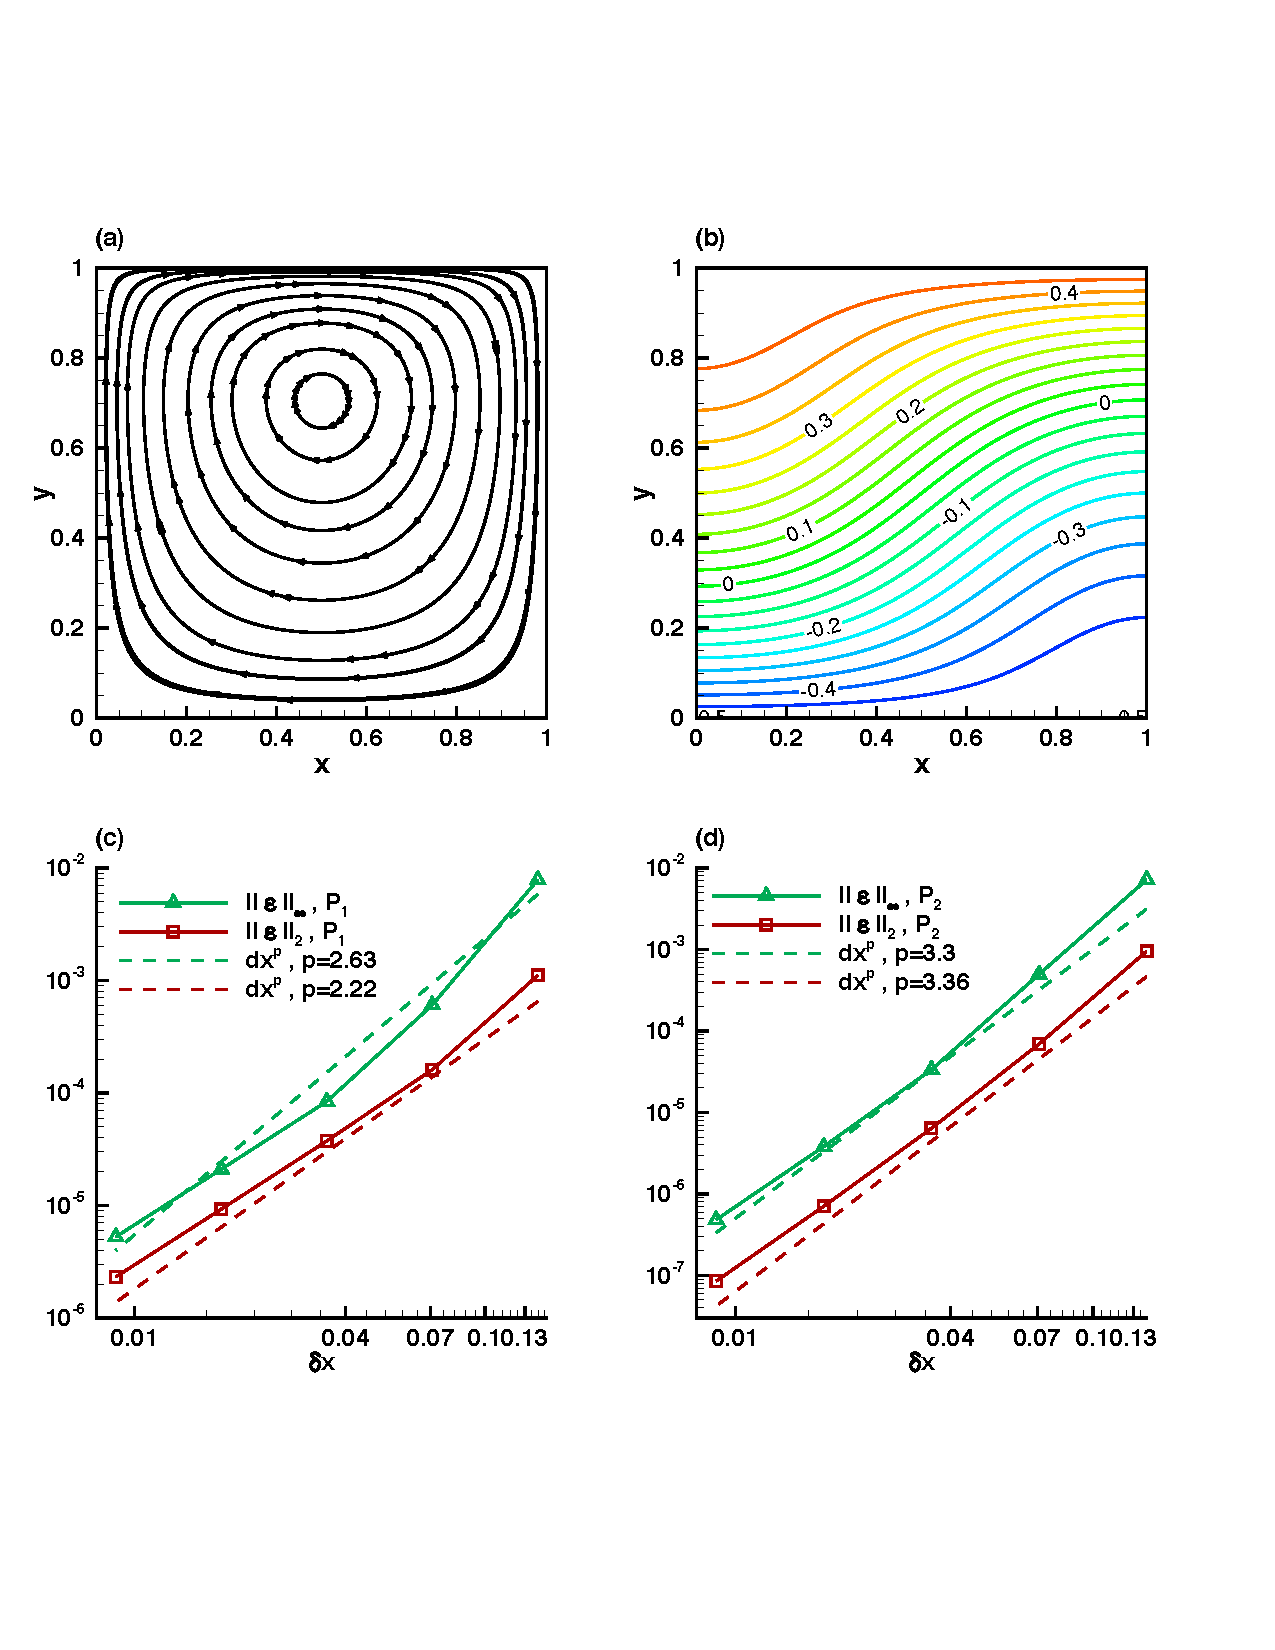
\includegraphics[width=\textwidth]{\figpath/Fig_cap_2/figsCPC_03} 
	\end{center}
	\caption{Burggraf stationary flow with thermal effects used to test the space accuracy of the numerical scheme. Streamlines (a) and temperature contours (b) of the flow field.	
Global error $\varepsilon$ (cf. Eq. (\ref{eq-epsconv})) for  the temperature: (c) P$_1$ and (d) P$_2$ finite elements.}
	\label{fig-conv-burggraf}
\end{figure}

%\pagebreak
%%%%%%%%%%%%%%%%%%%%%%%%%%%%%%%%%%%%%%%%%%%
\section{Time accuracy: manufactured unsteady solution} \label{subsub-conv-nourg}

To test the time accuracy of the Gear (BDF2) scheme, we used the manufactured time-dependent solution suggested in \cite{nourgaliev2016fully}:
\begin{align}
\label{eq-manufN}
	u_1(x,y,t) &=& \left( \delta U_0 + \alpha_u \, \sin(t) \right) \, \cos(x+ \gamma_1 t) \, \sin(y+ \gamma_2 t), \\ \nonumber
	u_2(x,y,t) &=& - \left( \delta U_0 + \alpha_u \sin(t) \right) \, \sin(x+ \gamma_1 t) \, \cos(y+ \gamma_2 t), \\ \nonumber
	T(x,y,t) &=& \bar{T} + \left( \delta T_0 + \alpha_t \sin(t) \right) \, \cos(x+ \gamma_1 t) \, \sin(y+ \gamma_2 t), \\ \nonumber
	p(x,y,t) &=& \bar{P} + \left(\delta P_0 + \alpha_p \sin(t) \right) \, \sin(x+ \gamma_1 t) \, \cos(y+ \gamma_2 t), 
\end{align}
The values of the constants are reported in Table \ref{tab-constant}.
\begin{table}[!h]
\centering
\begin{tabular}{*{10}{c}}
 % \toprule
  $\gamma_1$ & $\gamma_2$ & $\bar{P}$ & $\bar{T}$ & $\delta P_0$ & $\delta T_0$ & $\delta U_0$ & $\alpha_p$ & $\alpha_u$ & $\alpha_t$\\
   \midrule
  $0.1$ & $0.1$ & $0$ & $1.0$ &  $0.1$ & $1.0$ & $1.0$ & $0.05$ & $0.4$ & $0.1$ \\
 % \bottomrule
 \end{tabular}
\caption{Parameter for the time-dependent manufactured solution (\ref{eq-manufN}).}
\label{tab-constant}
\end{table}
The corresponding forcing source terms are:
\begin{eqnarray}
	f_{u_1} &=& \alpha_u \, \cos(t) \, \cos(a) \sin(b) - U_c \, \gamma_1 \, \sin(a) \sin(b) + U_c \, \gamma_2  \, \cos(a)\cos(b) \\ \nonumber
	  & & - U_c \,  u_1(x,y,t) \, \sin(a) \sin(b) + U_c \,  u_2(x,y,t) \, \cos(a) \cos(b)
	  + P_c \, \cos(a) \cos(b)\\ \nonumber
	  & & + \frac{2}{Re} \, u_1(x,y,t), \\	  \nonumber
	f_{u_2} &=& - \alpha_u \,  \cos(t)  \, \sin(a) \cos(b) - U_c \,  \gamma_1  \,  \cos(a) \cos(b) + U_c \,  \gamma_2 \,  \sin(a)\sin(b) \\ \nonumber
		  & & - U_c \,  u_1(x,y,t)  \,  \cos(a) \cos(b) + U_c  \, u_2(x,y,t)  \,  \sin(a) \sin(b)
		  -  P_c  \,  \sin(a)  \,  \sin(b)\\ \nonumber
		  & &+ \frac{2}{Re} \,  u_2(x,y,t)
		  - \frac{Ra}{Pr Re^2} \,  T(x,y,t), \\  \nonumber
	f_{T} &=& \alpha_t \,  \cos(t) \,  \cos(a) \sin(b) -  T_c  \,  \gamma_1 \,  \sin(a) \sin(b) + T_c \,   \gamma_2  \,  \cos(a)\cos(b) \\ \nonumber
		  & &-  T_c \,  u_1(x,y,t)  \,  \sin(a) \sin(b)  
		  +   T_c  \,  u_2(x,y,t)  \, \cos(a) \cos(b) 
		  + \frac{2 K}{Re Pr} \,  T_c  \, \cos(a) \sin(b), \\ \nonumber
\end{eqnarray}
where $a = (x+ \gamma_1 t), \,
b = (y+ \gamma_2 t)$ and  
$U_c = (\delta U_0 + \alpha_u \sin(t)), \,
	T_c = (\delta T_0 + \alpha_u \sin(t)), \,
	P_c = (\delta P_0 + \alpha_u \sin(t))$.

Guided by  the results obtained  in \S \ref{subsub-conv-burg} for the space accuracy, we fixed the grid size to $h=dx = 0.01$ to ensure small spatial discretization errors.
For diminishing values of the time step $\delta t$, the solution was evolved in time up to the time instant $t_{max} = \pi$ at which the error  (\ref{eq-epsconv}) was computed. 
The time convergence is displayed in Figure \ref{fig-conv-bdf2} for the temperature variable. 
The expected second order convergence in time is obtained for both P$_1$ (Figure \ref{fig-conv-bdf2}a) and P$_2$ (Figure \ref{fig-conv-bdf2}b) discretizations of the temperature.

\begin{figure}[!h]
	\begin{center}
		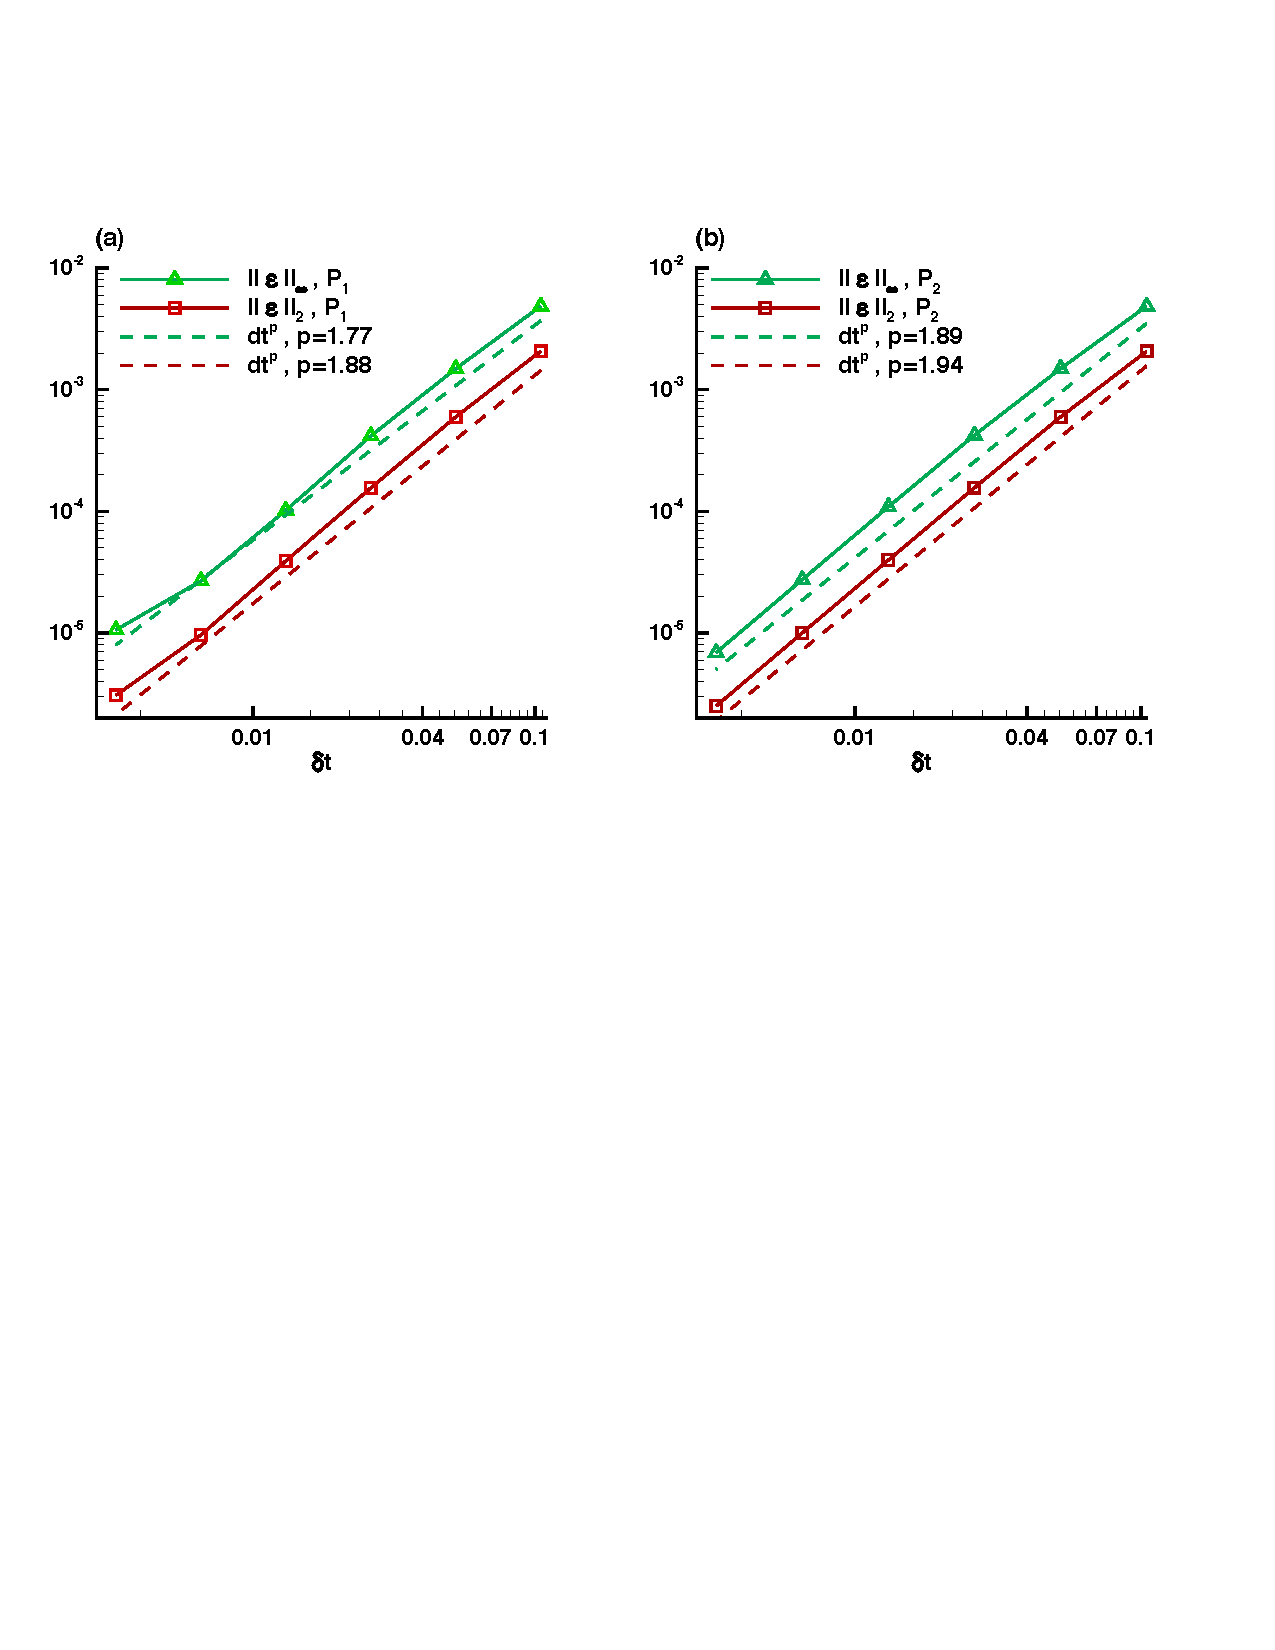
\includegraphics[width=\textwidth]{\figpath/Fig_cap_2/figsCPC_04} 
	\end{center}
	\caption{Time accuracy of the numerical scheme tested using the time-dependent manufactured solution of \cite{nourgaliev2016fully}. Evolution of the global error $\varepsilon$ given in (\ref{eq-epsconv}) for  the temperature at $t_{max} = \pi$. Discretizations using: (a) P$_1$ and (b) P$_2$ finite elements.}
	\label{fig-conv-bdf2}
\end{figure}


%\section{Accuracy and convergence} \label{subsec-conv}
%We test the accuracy of our numerical method in this section.
%Both space and time convergence orders are demonstrated by using the Burggraf flow and a manufactured solution defined by \cite{nourgaliev2016fully} for the incompressible Navier-Stokes equations.
%The global error $ \| \varepsilon_h \|$ is defined as follows:
%
%\begin{equation}
%  \| \varepsilon_h \| = \| \Phi_e - \phi_h \|,
%\end{equation}
%where $\Phi_e$ is the exact solution and $\phi_h$ is the numerical solution.
%Thus, by computing $\| \varepsilon_h \|$ for either different grids or different time steps, one can evaluate the convergence order $p$, since it is represented by the slope of the corresponding curve in logarithmic coordinates.
%
%Computations are done for the convection of air, with a Rayleigh number $Ra = 10^6$ and a Prandtl number $Pr = 0.71$.
%
%\subsection{Burggraf flow} \label{subsub-conv-burg}
%
%\begin{figure}
%	\begin{center}
%		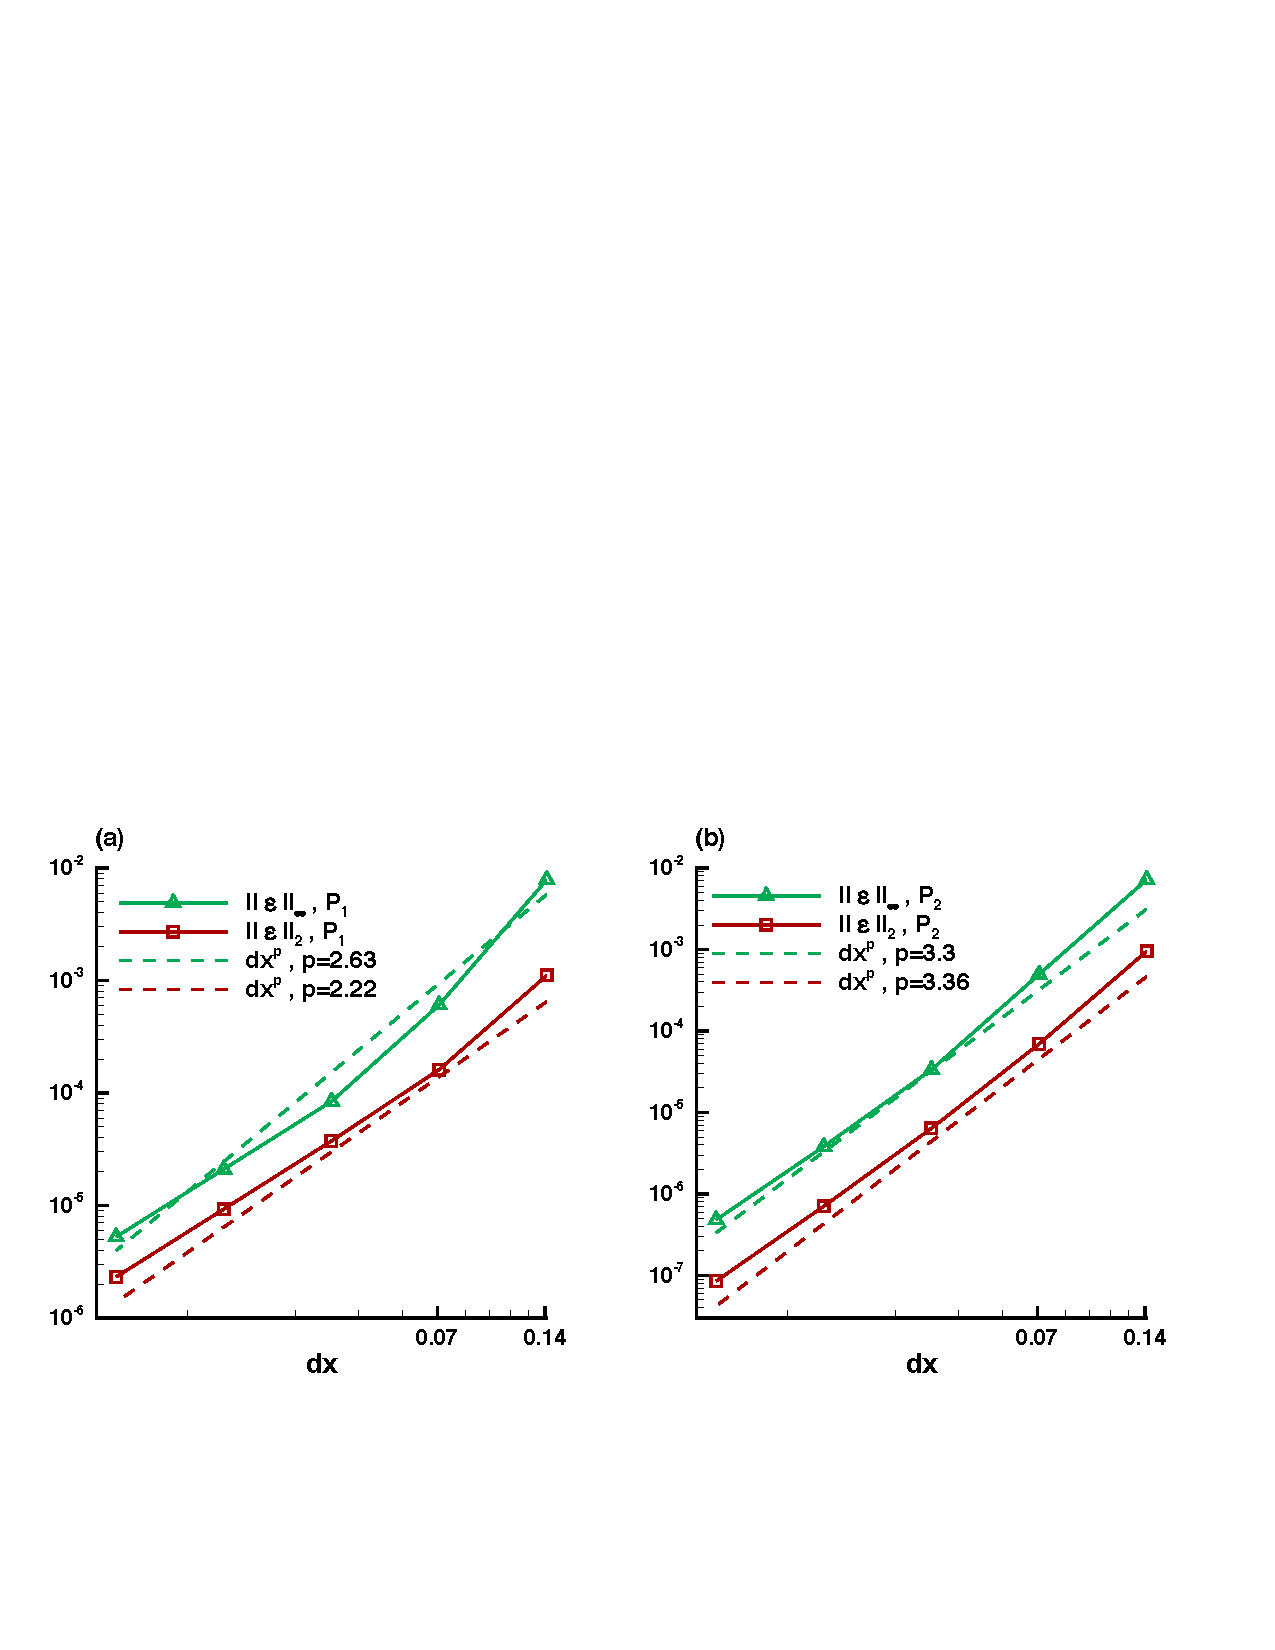
\includegraphics[width=0.98\textwidth]{\figpath/Fig_cap_2/Convergence_BURGGRAF} 
%	\end{center}
%	\caption{Burggraf flow. Evolution of the global error $\| \varepsilon_h \|$ for both $\mathcal{L}_2$-norm and $\mathcal{L}_\infty$-norm, with different grid size. A Taylor-Hood finite element (P$_2$ for velocity and P$_1$ for pressure) is used for space discretization by taking either P$_1$ finite element (a) or P$_2$ finite element (b) for the temperature field.}
%	\label{fig-conv-burggraf}
%\end{figure}
%
%To demonstrate the space accuracy of our method, we compute the well-known analytical solution called the Burggraf flow.
%It consists of a steady recirculating flow in a square cavity $[ 0 , 1] \times [ 0 , 1]$, with a moving wall at the top boundary and non-slip wall conditions at the others :
%
%\begin{eqnarray}
%   u(x,0) &=& u(0,y) = u(1,y) = 0, \\
%   u(x,1) &=& \sigma (x^4 - 2x^3 + x^2).
%\end{eqnarray}
%Besides, constant temperatures are imposed at the top and the bottom walls, while others are assumed to be adiabatic.
%The exact solution of the flow is:
%\begin{eqnarray}
%   u1(x,y) &=& \sigma g'(x) h'(y), \\\nonumber
%   u2(x,y) &=& - \sigma g''(x) h(y), \\\nonumber
%   p(x,y)   &=& \frac{\sigma}{Re} \left( h^{(3)}(y) g(x) + g''(x)h'(y) \right) + \frac{\sigma}{2} g'(x)^2 \left( h(y)h''(y)-h'(y)^2 \right),\\ \nonumber
%   T(x,y) &=& T_{c} + (T_{h} - T_{c}) y + a(x) b(y), \\ \nonumber
%\end{eqnarray}
%with,
%\begin{eqnarray}
%   g(x) &=& \frac{x^5}{5} - \frac{x^4}{2} - \frac{x^3}{3}, \\ \nonumber
%   h(y) &=& y^4 - y^2, \\ \nonumber
%   a(x) &=& \cos (\pi x), \\ \nonumber
%   b(x) &=& y(1-y).
%\end{eqnarray}
%Hence, forcing term are defined as follows:
%
%\begin{eqnarray}
%   f_{u1} &=& 0 \\ \nonumber
%   f_{u2} &=& \sigma^2 h(y) h'(y) \left( g''(x)^2 - g'(x)g^{(3)}(x) \right) \\ \nonumber
%   &+& \frac{\sigma}{Re}\left( g^{(4)}(x) h(y) + 2 g''(x)h''(y) + g(x) h^{(4)}(y) \right) \\ \nonumber
%   &+& \frac{\sigma^2}{2} g'(x)^2 \left( h(y) h^{(3)}(y) - h'(y)h''(y) \right) - \frac{Ra}{Pr Re^2} T(x,y),\\ \nonumber
%   f_T &=& u1(x,y) a'(x) b(y) + u2(x,y) \left( T_h - T_c + a(x) b'(y) \right) \\ \nonumber
%   &-& \frac{K}{Re Pr} \left( a''(x)b(y) + a(x) b''(y) \right).
%\end{eqnarray}
%We use the Taylor-Hood finite element (P$_2$ for velocity and P$_1$ for pressure) for the space discretization with either P$_1$ or P$_2$ finite element for the temperature field.
%Figure \ref{fig-conv-burggraf} plots the decrease of the global discretization error $\| \varepsilon_h \|$ for both $\mathcal{L}_2$-norm and $\mathcal{L}_\infty$-norm function of the grid size.
%The expected second order convergence is obtained with a P$_1$ finite element for the temperature (Figure \ref{fig-conv-burggraf}a), and even a nearly third order is noticed with a P$_2$ finite element on the temperature (Figure \ref{fig-conv-burggraf}b).
%
%\subsection{Manufactured solution} \label{subsub-conv-nourg}
%\begin{figure}
%	\begin{center}
%		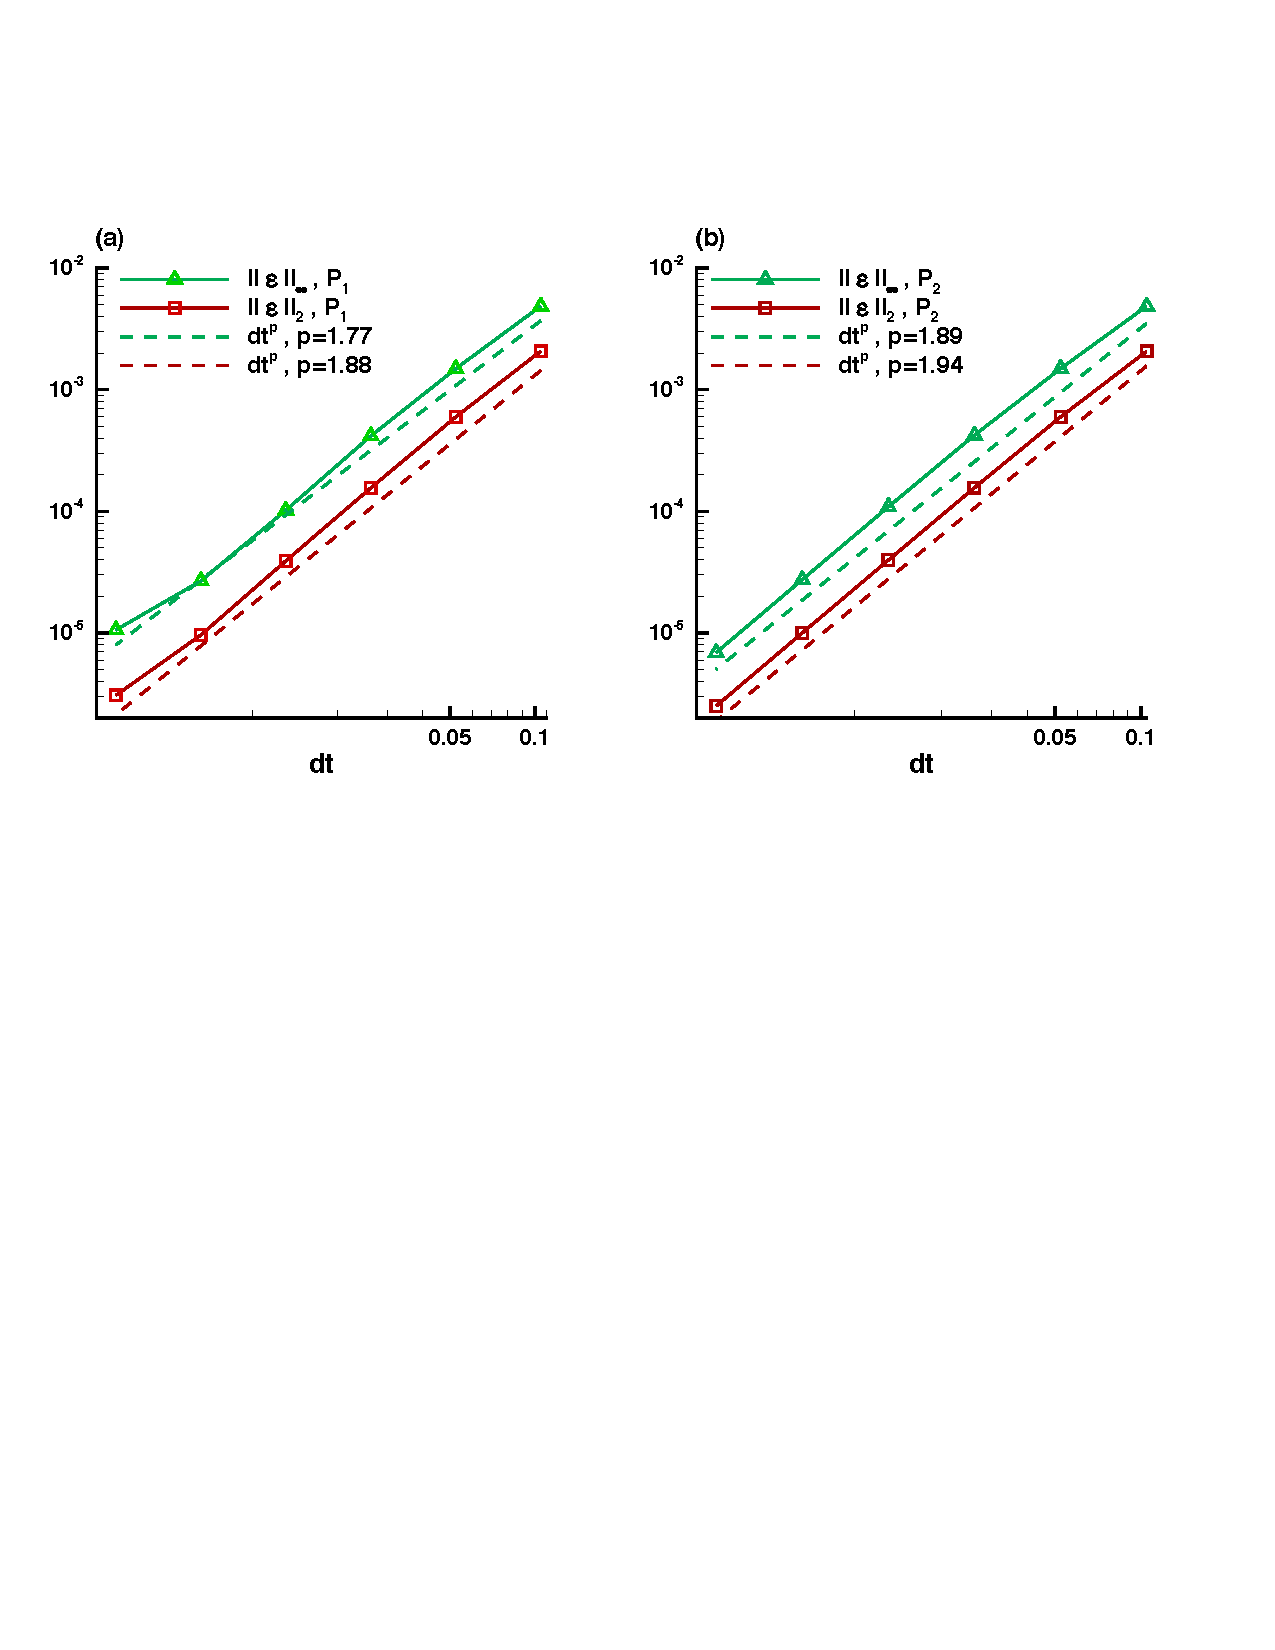
\includegraphics[width=0.98\textwidth]{\figpath/Fig_cap_2/Convergence_BDF2} 
%	\end{center}
%	\caption{Manufactured solution of \cite{nourgaliev2016fully} for unsteady incompressible Navier-Stokes equation at dimensionless time $t = \pi$. Evolution of the global error $\| \varepsilon_h \|$ for both $\mathcal{L}_2$-norm and $\mathcal{L}_\infty$-norm, with different time steps, with a P$_1$ finite element (a) and a P$_2$ finite element (b) for the temperature.}
%	\label{fig-conv-bdf2}
%\end{figure}
%
%The time integration is based on the implicit second order scheme BDF2.
%We use the manufactured solution of \cite{nourgaliev2016fully} to measure the temporal convergence order.
%\begin{eqnarray}
%	u_1(x,y,t) &=& \left( \delta U_0 + \alpha_u \, \sin(t) \right) \, \cos(x+ \gamma_1 t) \, \sin(y+ \gamma_2 t), \\ \nonumber
%	u_2(x,y,t) &=& - \left( \delta U_0 + \alpha_u \sin(t) \right) \, \sin(x+ \gamma_1 t) \, \cos(y+ \gamma_2 t), \\ \nonumber
%	T(x,y,t) &=& \bar{T} + \left( \delta T_0 + \alpha_t \sin(t) \right) \, \cos(x+ \gamma_1 t) \, \sin(y+ \gamma_2 t), \\ \nonumber
%	p(x,y,t) &=& \bar{P} + \left(\delta P_0 + \alpha_p \sin(t) \right) \, \sin(x+ \gamma_1 t) \, \cos(y+ \gamma_2 t), 
%\end{eqnarray}
%The value of the constants are reported on Table \ref{tab-constant}.
%\begin{table}[!h]
%\centering
%\begin{tabular}{*{10}{c}}
% % \toprule
%  $\gamma_1$ & $\gamma_2$ & $\bar{P}$ & $\bar{T}$ & $\delta P_0$ & $\delta T_0$ & $\delta U_0$ & $\alpha_p$ & $\alpha_u$ & $\alpha_t$\\
%   \midrule
%  $0.1$ & $0.1$ & $0$ & $1.0$ &  $0.1$ & $1.0$ & $1.0$ & $0.05$ & $0.4$ & $0.1$ \\
% % \bottomrule
%
% \end{tabular}
%\caption{Parameter for the manufactured solution.}
%\label{tab-constant}
%\end{table}
%
%\noindent Thus, forcing terms are:
%
%\begin{eqnarray}
%	f_x &=& \alpha_u \, \cos(t) \, \cos(a) \sin(b) - U_c \, \gamma_1 \, \sin(a) \sin(b) + U_c \, \gamma_2  \, \cos(a)\cos(b) \\ \nonumber
%	  & & - U_c \,  u_1(x,y,t) \, \sin(a) \sin(b) + U_c \,  u_2(x,y,t) \, \cos(a) \cos(b)
%	  + P_c \, \cos(a) \cos(b)\\ \nonumber
%	  & & + \frac{1}{Re} \, u(x,y,t), \\	  \nonumber
%	f_y &=& - \alpha_u \,  \cos(t)  \, \sin(a) \cos(b) - U_c \,  \gamma_1  \,  \cos(a) \cos(b) + U_c \,  \gamma_2 \,  \sin(a)\sin(b) \\ \nonumber
%		  & & - U_c \,  u_1(x,y,t)  \,  \cos(a) \cos(b) + U_c  \, u_2(x,y,t)  \,  \sin(a) \sin(b)
%		  -  P_c  \,  \sin(a)  \,  \sin(b)\\ \nonumber
%		  & & -\frac{1}{Re} \,  v(x,y,t)
%		  - \frac{Ra}{Pr Re^2} \,  T(x,y,t), \\  \nonumber
%	f_{\theta} &=& \alpha_t \,  \cos(t) \,  \cos(a) \sin(b) -  T_c  \,  \gamma_1 \,  \sin(a) \sin(b) + T_c \,   \gamma_2  \,  \cos(a)\cos(b) \\ \nonumber
%		  & &-  T_c \,  u_1(x,y,t)  \,  \sin(a) \sin(b)  
%		  +   T_c  \,  u_2(x,y,t)  \, \cos(a) \cos(b) 
%		  + \frac{K}{Re Pr} \,  T_c  \, \cos(a) \sin(b), \\ \nonumber
%\end{eqnarray}
%
%with: 
%$	U_c = (\delta U_0 + \alpha_u \sin(t)), \,
%	T_c = (\delta T_0 + \alpha_u \sin(t)), \,
%	P_c = (\delta P_0 + \alpha_u \sin(t)), $ \\
%and $	a = (x+ \gamma_1 t), \,
%	b = (y+ \gamma_2 t). \\$
%
%Since the space convergence rate was evaluated in \S \ref{subsub-conv-burg}, we fixe the grid size to $dx = 0.01$ to ensure a small spatial discretization errors, and we vary decreasingly the time step.
%Time convergence is displayed in Figure \ref{fig-conv-bdf2}. 
%The evolution of the global error with different time steps is plotted for both  $\mathcal{L}_2$-norm (red line) and $\mathcal{L}_\infty$-norm (green line), and the expected second order convergence is exposed for both P$_1$ (Figure \ref{fig-conv-bdf2}a) and P$_2$ (Figure \ref{fig-conv-bdf2}b) finite element for the temperature.

%\newpage
%\section{A finite-element toolbox for the simulation of phase-change systems with natural convection}\label{sec-desc-prog}
%
%The methods described previously were implemented in a 2D toolbox based on \ff software.
%%Using two input files, the toolbox offers to the user the choice between three scalings in order to compute different physical systems involving natural convection flow, ranging from natural convection of air and water to melting and solidification cycle of PCM or water freezing.
%%The solutions can be saved at recurrent iterations defined by the user beforehand, allowing later to restart the computation from  saved solutions.
%In this section we first describe the architecture of the programs and the organisation of files.
%Then we focus on the list of input parameters and the structure of output files.
%%
%\begin{figure}[!h]
%	\begin{center}
%		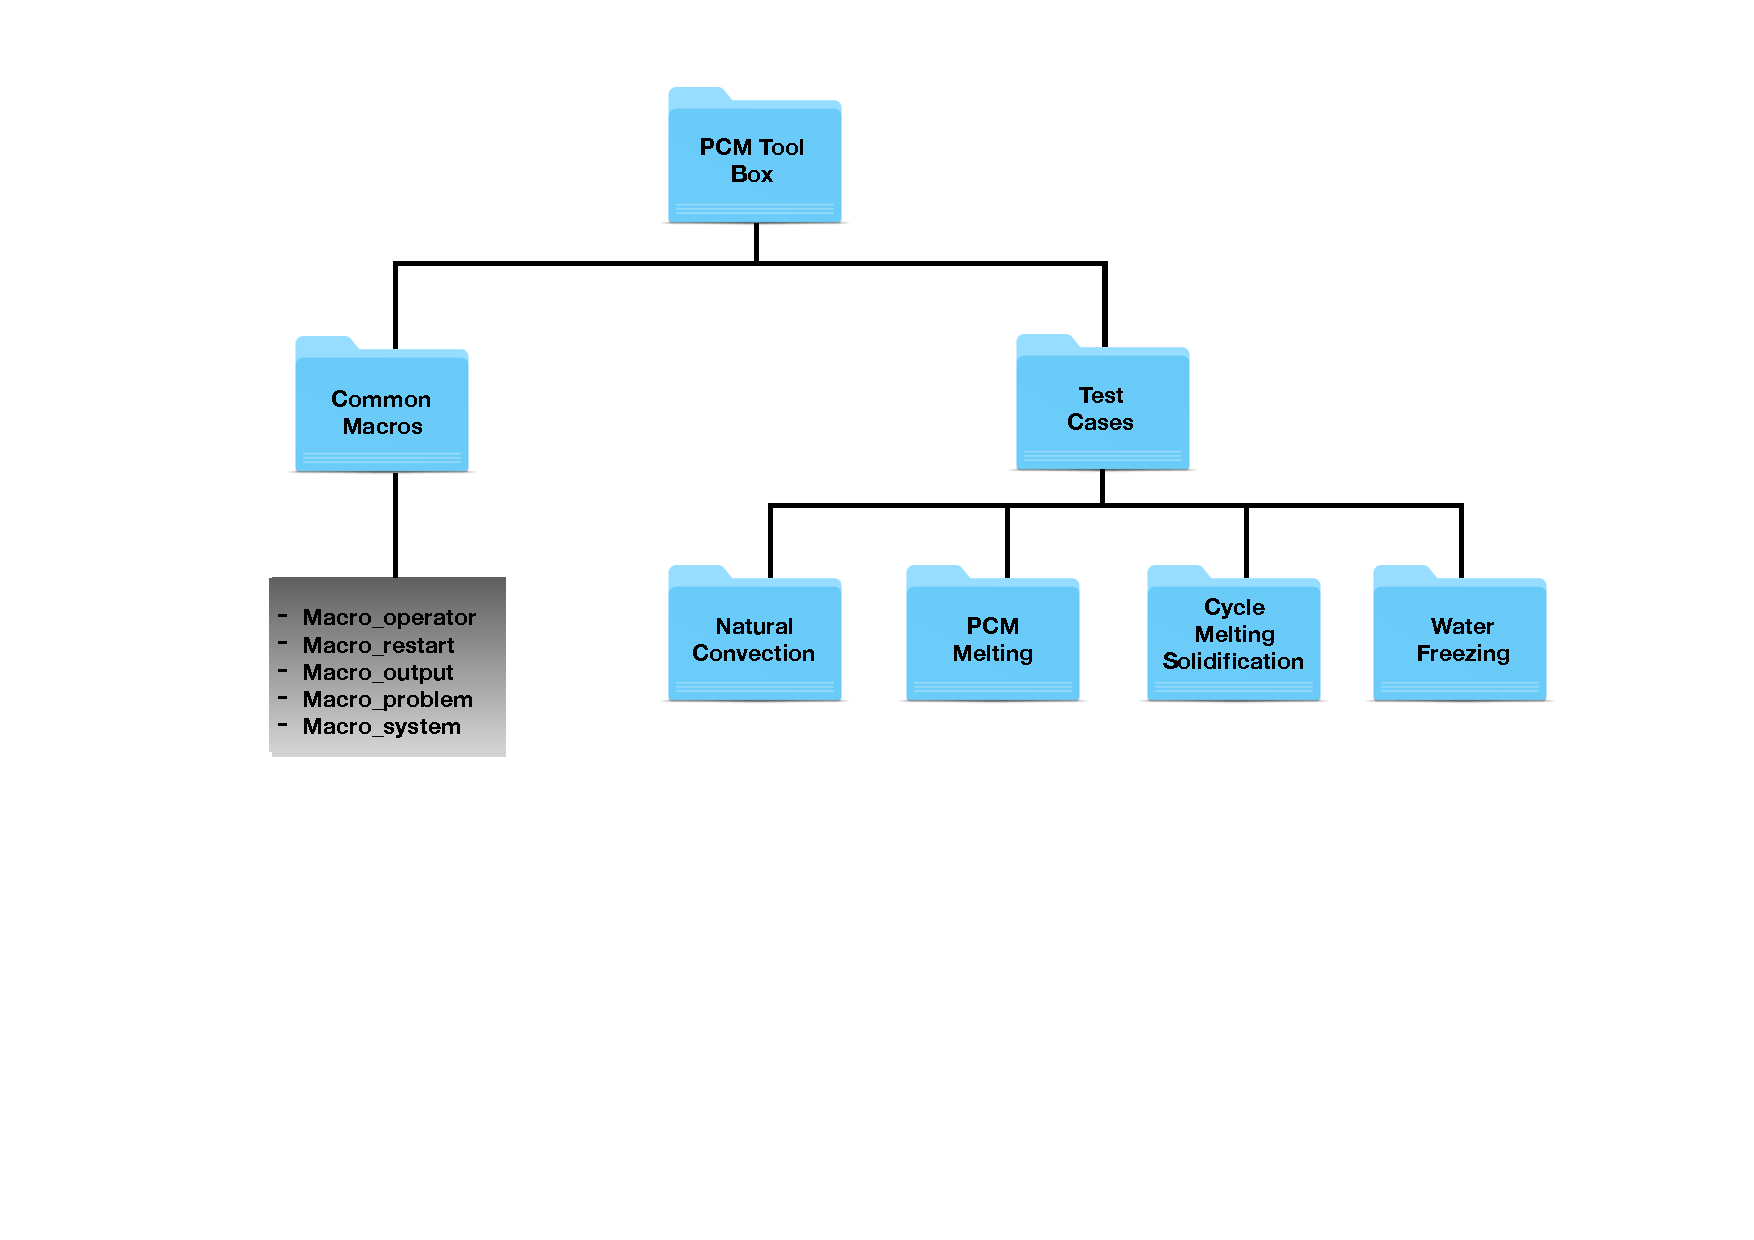
\includegraphics[width=0.9\textwidth]{\figpath/Fig_cap_2/FOLDER_arbor_3}
%	\end{center}
%	\caption{Folder tree structure of the FreeFem++ toolbox to solve phase change problems. Test cases and common macros are separated into two folders.}
%	\label{fig-folder-tree}
%\end{figure}
%
%\subsection{Program architecture}
%Figure \ref{fig-folder-tree} gives a schematic overview of the content of the toolbox. All files are provided in a directory called \texttt{PCM-Toolbox}.  Many detailed comments are included in the programs, with direct link to the mathematical expressions used in the paper. The used \ff syntax was intentionally kept at a low level of technicality and supplemented with detailed comments when specific more technical syntax was used.
%
%This directory is organized as follows:
%\begin{enumerate}
%   \item The directory \texttt{Common-Macros} contains five files:\\
%$\bullet$ {\em Macro$\_$operator.idp} includes macros and functions defining mathematical operators,\\
%$\bullet$ {\em Macro$\_$problem.idp}: macros defining the variational formulation of the problem,\\
%$\bullet$ {\em Macro$\_$restart.idp}: macros used to start a new simulation from a saved field,\\
%$\bullet$ {\em Macro$\_$output.idp}: macros used to save the solution with different formats,\\
%$\bullet$ {\em Macro$\_$system.idp}: macros identifying the OS and defining specific OS-commands.
%
%   \item The directory \texttt{Test-Cases}  contains four subdirectories, each of them defining one of the following applications:\\
%    $\bullet$  natural convection of air or water in a differentially heated square cavity, \\
%    $\bullet$  melting of a PCM stored in containers of different shapes,\\
%    $\bullet$  melting followed by solidification of a rectangular PCM,\\
%    $\bullet$  freezing of pure water in a square cavity.\\
%   Each subdirectory contains  three files: {\em NEWTON$\_$\$case.edp} is the main \ff script file, $param_\_phys.inc$ defines the physical parameters and $param_\_num.inc$ the numerical parameters. For example, to run the natural convection case of air in a square cavity, the user can use the following command in a terminal window:
%  \texttt{FreeFem++ NEWTON$\_$stat$\_$natconv.edp}.\\
%  The folder structure of each test case is illustrated in Figure \ref{fig-case-folder}.
%  The obtained solutions are saved in the folder \texttt{OUTPUT/Data}. Depending on the output format selected by the user,  data files are generated in specific folders for being visualized with: Tecplot, Paraview, Gnuplot or Medit. We also provide in the folder \texttt{Figures} ready-made layouts for these visualisation softwares. The user can thus obtain the figures from this paper using  newly generated data. More details about the output structure are given below.
%\end{enumerate}
%
%\begin{figure}[!h]
%	\begin{center}
%		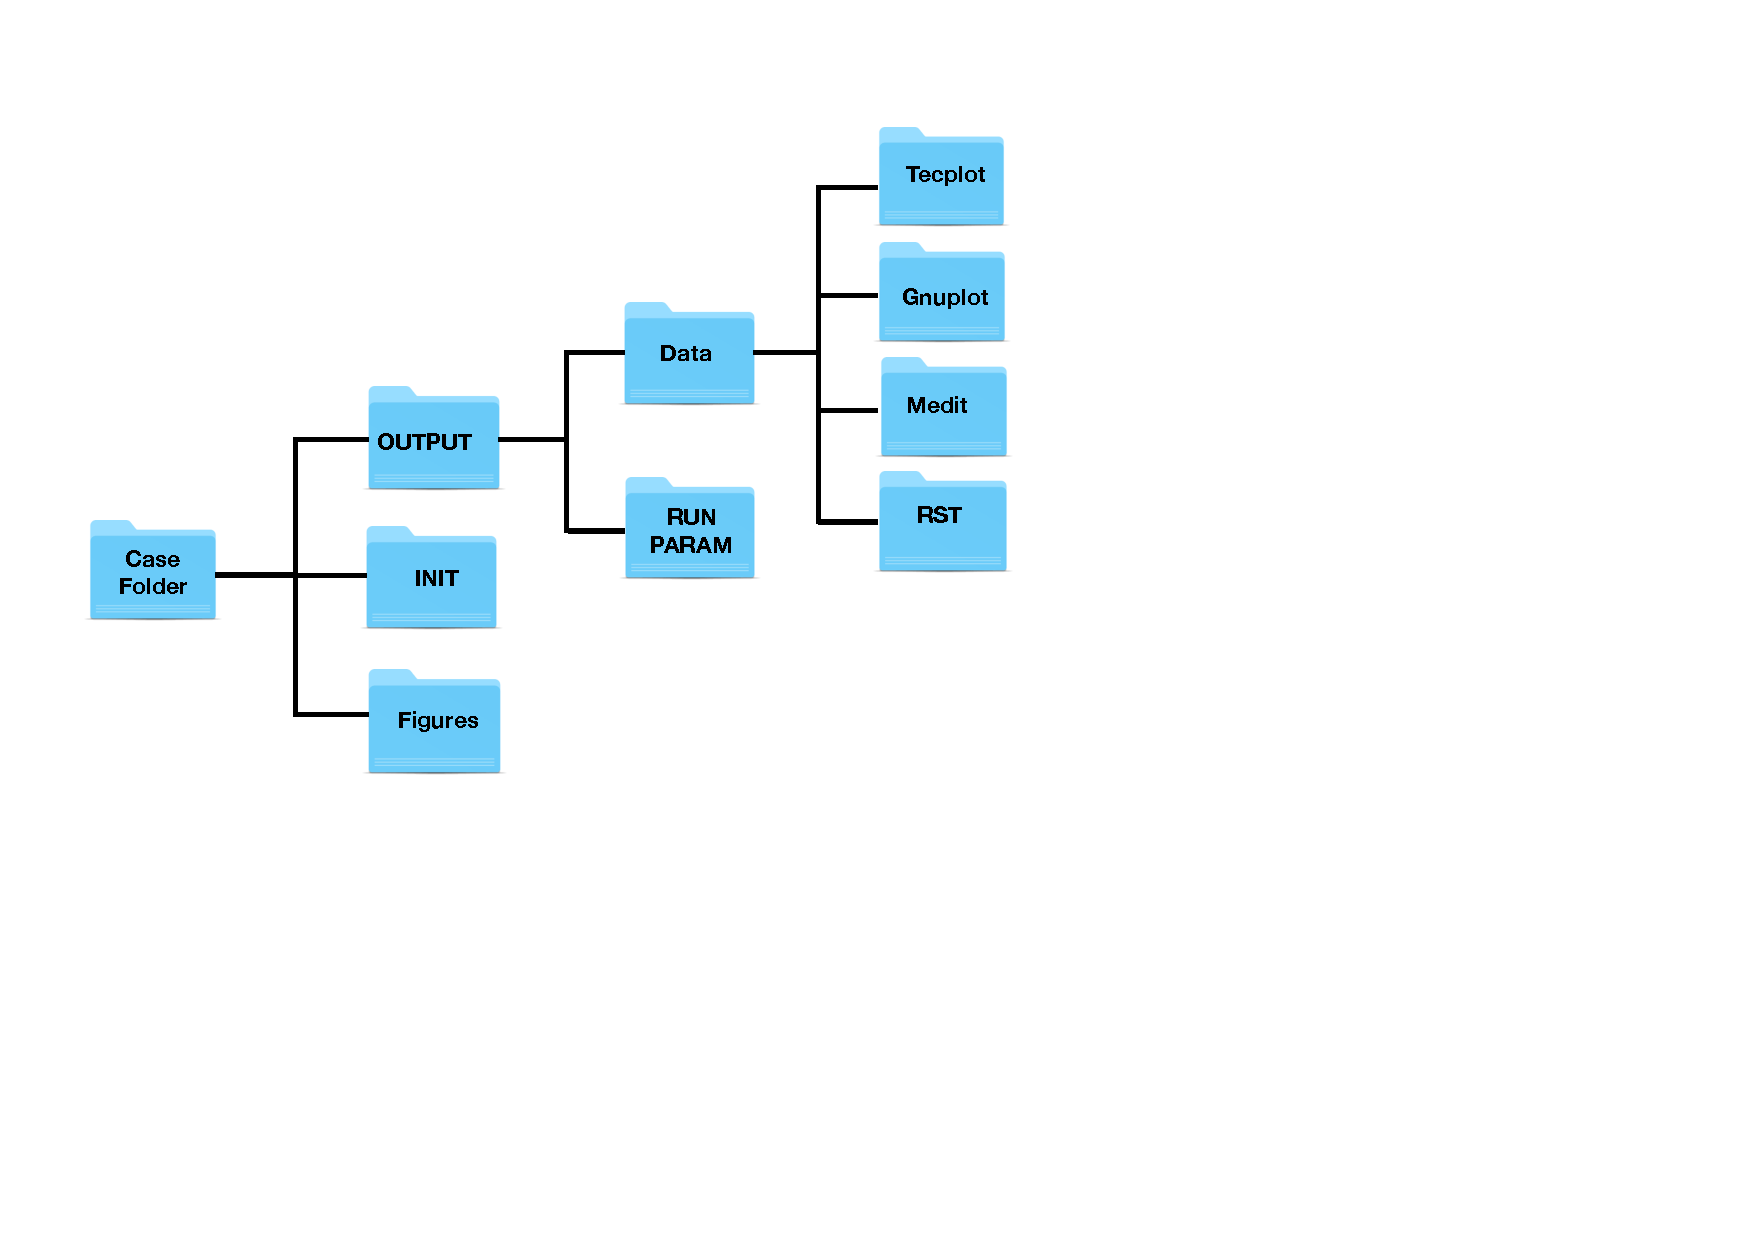
\includegraphics[width=0.7\textwidth]{\figpath/Fig_cap_2/figsCPC_02}
%	\end{center}
%	\caption{Structure of each Test-case folder. 
%	}
%	\label{fig-case-folder}
%\end{figure}
%
%\subsection{Input parameters}
%
%Physical parameters and parameters related to the run are separated into two files.\\
%{\bf (1)} The file $param_\_phys.inc$ contains the physical descriptions of the problem:
%\begin{itemize}
%   \item {\bf typeT}: is the finite-element type for the temperature, with possible values \texttt{P2} or \texttt{P1},
%   \item {\bf Torder}: is the accuracy order of the time integration scheme, with possible values $1$ (Euler scheme) or $2$ (Gear scheme),
%   \item {\bf scalAdim}: defines the characteristic scales of the problem, see (\ref{eq-adim}). Possible values 1, 2 or 3 correspond to the following choice of the characteristic scales \citep{dan-2014-JCP}:
%   \begin{eqnarray} \label{eq-scal1}
%    (1) &:&  V_\vref^{(1)} = \frac{\nu_l}{H} \Longrightarrow \ds t_\vref^{(1)} = \frac{H^2}{\nu_l}  \Longrightarrow \Rey=1,\\
%      \label{eq-scal2}
%     (2) &:& V_\vref^{(2)} = \frac{\alpha}{H} \Longrightarrow \ds t_\vref^{(2)} = t_\vref^{(1)} \Prd  \Longrightarrow \Rey =1/\Prd,\\
%      \label{eq-scal3}
%     (3) &:& V_\vref^{(3)} = \frac{\nu_l}{H} \sqrt{\frac{\Ray}{\Prd}} \Longrightarrow \ds t_\vref^{(3)} = t_\vref^{(1)} \sqrt{\frac{\Prd}{\Ray}}       \Longrightarrow \Rey = \sqrt{\frac{\Ray}{\Prd}},
%\end{eqnarray}
%   \item {\bf x$_l$, x$_r$, y$_l$, y$_r$}: are the values defining the dimensions of the cavity $[x_l,x_r]\times[y_l,y_r]$,
%   \item {\bf Pr, Ra, Ste}: are the  Prandtl, Rayleigh and Stefan numbers, see (\ref{eq-Rayleigh}) and (\ref{eq-RePr}),
%   \item {\bf T$_{hot}$, T$_{cold}$}: are  dimensionless temperatures according to (\ref{eq-adim}),
%   \item{\bf bcu$_1$, bcu$_2$, bcT}: are macros defining the velocity (u) and the temperature (T) boundary conditions.
%   \item {\bf epsi}: is the half width $\varepsilon$ of the mushy region. \underline{Default value} = $0.01$,
%   \item {\bf dt}: is the dimensionless time step,
%   \item {\bf t$_{max}$}: is the dimensionless final time,
%   \item {\bf Parameters for regularization functions}: \\
% The parameters of the hyperbolic-tangent function (\ref{eq-smooth}) used to regularize discontinuous functions are set by default as follows:
% \end{itemize}
%    \begin{table}[!ht]
%    \centering
%    \begin{tabular}{*{8}{c}}
%     & { f$_{s}$} & {f$_{l}$} & {a$_s$} & {$\theta_s$} & R$_s$ & {$\CKC$} & {b} \\
%       \toprule
%       {\it Enthalpy} & 0 & 1/Ste & 1 & 0.01 & 0.01  & - & - \\
%       \midrule
%       {\it Carman - Kozeny} & 0 & 1 & 1 & 0.01 & 0.01  & 10$^6$ & 10$^{-7}$ \\
%          \midrule
%       {\it Conductivity (water)} & 1 & 2.26/0.578 & 1 & $\theta_f$ & 0.015 & - & - \\
%       \bottomrule
%     \end{tabular}
%    \label{tab-constant}
%    \end{table}
%   \begin{itemize} 
%    \item {\bf rho(T) and Drho(T)}: (water cases only) define  the density and its derivative as functions of the temperature, following the model
%\citep{Gebhart1977}:\\
% 
%    \begin{table}[!ht]
%    \centering
%    \begin{tabular}{*{4}{c}}
%    	\multicolumn{4}{c}{
%      $\rho(T) = \rho_m (1 - \omega | T - T_m |^q),$}\\	\hline
%    $\rho_m$ [kg/m$^3$]  & $\omega$ [$^o$C$^{-q}$] & q & $T_m$  [$^o$C] \\
%       \toprule
%            $999.972$ & $9.2793 \cdot 10^{-6}$ & $1.894816$ & $4.0293$ \\
%       \bottomrule
%     \end{tabular}
%    \label{tab-rho}
%    \end{table}
%    \item {\bf f$_B$(T), df$_B$(T)}: define the buoyancy force and its derivative.
%    \end{itemize}
%
%\noindent {\bf (2)} The file {\em param$\_$num.inc} contains the parameters controlling the run.\\
%{\bf Restart parameters:}
%\begin{itemize}
%   \item {\bf Nsave}: the solution is saved every $N\!save$ time steps in the \texttt{Data} folder (see Figure \ref{fig-case-folder}). The temperature and the velocity fields are saved in \texttt{Tecplot} and \texttt{Medit} folders, while the liquid fraction, the Nusselt number, and the accumulated heat input are saved in the \texttt{Gnuplot} folder.
%   \item {\bf Nrestart}: restart files (mesh and solution) are saved every $N\!restart$ time steps. Solutions at current and previous iterations, the CPU time, the accumulated heat input $Q_0$, and the time step $dt$ are saved in the folder \texttt{RST}.
%   \item {\bf Ncondt}: allows the user to stop the run and save the solution properly. The file \texttt{OUTPUT/zz.condt} is read every $N\!condt$ time steps: if the user replaces the value "0" in this file by "1" the run is stopped. This is a simple solution for a clean stop of the job by the user. \underline{Default value} = $20$.
%   \item {\bf Nremesh}: the mesh is adapted every $N\!remesh$ iterations. If this parameter is set to "1" the mesh is adapted every time step.
%   \item {\bf IFrestart}: is a boolean controlling the set up of the initial field. \\
%  $I\!Frestart = 0$, the  initial condition is built in the code for each test case. For the PCM melting cases, the PCM is initially motionless at isothermal temperature. 
%  	To set-up a smooth initial field, a few time steps (with very small $\delta t$) are computed by increasing progressively the boundary temperature at the hot wall and the Rayleigh number (by continuation).  Outputs are saved in  \texttt{OUTPUT/Data-RST-0}.\\
%   $I\!Frestart > 0$, (positive integer values) the solution field previously computed at iteration $I\!Frestart$ is loaded from the folder \texttt{OUTPUT/Data-RST-filenameRST/RST}, with \texttt{filenameRST} a variable selecting the restart folder. \\
%   $I\!Frestart < 0$, (negative integer values), the same principle for loading a solution is used, but from the folder \texttt{INIT}  (see Figure \ref{fig-case-folder}). The solution fields stored in this folder could come from different previous calculations (\eg a steady state solution or, for the water, the natural convection field before freezing).
%\end{itemize}
%
%{\bf Newton parameters:}
%\begin{itemize}
%   \item {\bf epsconv}: is the value of  the stopping criterion for steady cases,
%   \item {\bf gamma}: is the penalty parameter in  (\ref{eq-time-disc1}). \underline{Default value} = $10^{-7}$,
%   \item {\bf tolNewton}: is the Newton tolerance $\xi_N$ (see (\ref{eq-Newton-algo})). \underline{Default value} = $10^{-6}$,
%   \item {\bf newtonMax}: limits the maximum number of iterations in  the Newton algorithm (\ref{eq-Newton-algo}). \underline{Default value} = $50$,
%  % \Blue{\item {\bf c$_1$, c$_2$, c$_3$}: \Red{(-- why not negative $a_2$ ?? si c'est trop compliqu� de changer, il faut le laisser tel quel --$>$ } \Blue{C'est modifi� en a$_2$ n�gatif maintenant dans le code)--}  are the coefficients of the time integration scheme: c$_1 =1/$dt, c$_2 = -1/$dt, c$_3 = 0$ correspond to the first order backward Euler scheme and c$_1 =1.5/$dt, c$_2 = -2/$dt, and c$_3 = 0.5/$dt to the second order Gear scheme.}
%\end{itemize}
%{\bf Mesh parameters:}
%\begin{itemize}
%   \item {\bf nbseg}: is  the number of segments for the discretisation along the $x$ and $y$ directions,
%   \item {\bf errh}: is the interpolation error level. \underline{Default value} = $0.02$,
%   \item {\bf hmin, hmax}: are the minimum and maximum edge size, respectively,
%   \item {\bf adaptratio}: is the ratio for a prescribed smoothing of the metric. For a value less than $1.1$ no smoothing is done. \underline{Default value} = $1.5$,
%   \item {\bf nbvx}: is the maximum number of vertices allowed in the mesh generator. \underline{Default value} = $50000$.
%\end{itemize}
%
%\noindent {\bf Output parameters:}
%   \begin{itemize}
%      \item {\bf dircase}: is the name of the output folder,
%      \item {\bf fcase}: is the prefix-name for ouput files.
%      \item {\bf Tecplot, Medit, Gnu}: correspond to the name of the visualisation software to be used; the format of the outputs written in \texttt{OUTPUT/Data} (see Figure \ref{fig-case-folder}) is accordingly set.  The files from the Tecplot folder can be easily read  also with Paraview.
%   \end{itemize}
%   
%\subsection{Outputs}
%When a computation starts, the \texttt{OUTPUT} directory is created (see Figure \ref{fig-case-folder})).
%It contains two folders storing the output data and the echo of the run parameters.
%The folder \texttt{Data} contains four subdirectories with different output format files of the computed solution. File names are created using  the prefix defined by the parameter {\bf fcase}, the current iteration and the current dimensionless time $t$. 
%Solution files can be visualized using either Tecplot or any other CFD Visualization tools (Paraview, Visit, etc.). 
%Moreover, {\em .gmsh}  (mesh) and {\em .rst} (fields) files are generated in the folder \texttt{RST} to enable restarts of the computation. Note that the folder \texttt{FFglut} contains  \ff scripts that re-read and visualize the RST-files to facilitate the selection of a restart field.  
%An {\em .echo} file with a summary of the main parameters, informations on the run and the names of the output files is saved in the folder \texttt{RUNPARAM}.  This directory additionally contains a copy of the {\em .inc} parameter files, allowing an easy identification of each case and preparing an eventual rerun of the same case.
%
%
%%Figure \ref{fig-folder-tree} gives a schematic overview of the content of the toolbox. All files are provided in a directory called {\it "PCM ToolBox FreeFem"}. 
%%This directory is organized as follows:
%%\begin{enumerate}
%%   \item the {\em Common Macros} directory contains four files:
%%   \begin{itemize}
%%      \item {\em Macro$\_$operator.idp} contains all macros and functions related to mathematical operators,
%%      \item {\em Macro$\_$restart.idp} contains the scripts to be used to take the computation back from saved solutions,
%%      \item {\em Macro$\_$output.idp} contains the scripts allowing to output the solutions,
%%      \item {\em Macro$\_$problem.idp} contains the variational formulation of the problem. 
%%   \end{itemize}
%%   \item The {\em Test Cases} directory contains four subdirectories clustering different physical test cases, including the natural convection of air or water in a differentially heated square cavity, the melting of a PCM included in various containers, the melting-solidification cycle of a PCM and finally the freezing of pure water in a square cavity. 
%%   For all cited cases, three files are given for each subdirectories: {\em NEWTON$\_$\$case.edp} the main FreeFem++ script file, $param_\_phys.inc$ the physical parameters and $param_\_num.inc$ the numerical parameters.
%%   The natural convection case can be launched, for example, using the following command line in a terminal window:\\
%%  {\em FreeFem++ NEWTON$\_$airconv.edp -nbseg 80}.\\
%%  This will run the natural convection of air using $80 \times 80$ grids.
%%\end{enumerate}
%%
%%\subsection{Input parameters}
%%We focus now on the description of the input parameters.
%%The physical parameters and parameters related to the run are separated into two files.\\
%%{\bf (1)} First, the file $param_\_phys.inc$ contains the physical descriptions of the problem:
%%
%%\begin{itemize}
%%   \item {\bf typeT}: indicates the finite element type for the temperature. Choose between P$_1$ or P$_2$,
%%   \item {\bf scalAdim}: defines the characteristic scales of the problem. Choose between 1,2 or 3 \citep{dan-2014-JCP}:
%%   \begin{eqnarray} \label{eq-scal1}
%%    (1) &:&  V_\vref^{(1)} = \frac{\nu_l}{H} \Longrightarrow \ds t_\vref^{(1)} = \frac{H^2}{\nu_l}  \Longrightarrow \Rey=1,\\
%%      \label{eq-scal2}
%%     (2) &:& V_\vref^{(2)} = \frac{\alpha}{H} \Longrightarrow \ds t_\vref^{(2)} = t_\vref^{(1)} \Prd  \Longrightarrow \Rey =1/\Prd,\\
%%      \label{eq-scal3}
%%     (3) &:& V_\vref^{(3)} = \frac{\nu_l}{H} \sqrt{\frac{\Ray}{\Prd}} \Longrightarrow \ds t_\vref^{(3)} = t_\vref^{(1)} \sqrt{\frac{\Prd}{\Ray}}       \Longrightarrow \Rey = \sqrt{\frac{\Ray}{\Prd}},
%%\end{eqnarray}
%%   \item {\bf x$_0$, x$_l$, y$_0$, x$_l$}: correspond to the dimensions of the cavity.
%%   \item {\bf Pr, Ra, Ste}: are the dimensionless numbers Prandtl, Rayleigh and Stefan respectively defined in (\ref{eq-Rayleigh}) and (\ref{eq-RePr}),
%%   \item {\bf T$_{hot}$, T$_{cold}$}: denote the dimensionless temperatures according to (\ref{eq-adim}),
%%   \item{\bf bcu$_1$, bcu$_2$, bcT, bcp}: correspond to the velocity, the temperature and the pressure boundary conditions respectively.
%%   \item {\bf epsi}: expresses the half width $\varepsilon$ of the mushy region. \underline{Default value} = $0.01$,
%%   \item {\bf dt}: refers to the dimensionless time step,
%%   \item {\bf t$_{max}$}: fixes the dimensionless final time,
%%   \item {\bf Parameters for regularization functions}: \\
%% Parameters of the hyperbolic-tangent function used to regularize the discontinuous parameters are set by default as follows:
%% \end{itemize}
%%    \begin{table}[!ht]
%%    \centering
%%    \begin{tabular}{*{8}{c}}
%%     & {\bf f$_{{\hbox {\tiny S}}}$} & {\bf f$_{{\hbox {\tiny L}}}$} & {\bf as} & {\bf $\theta s$} & Rs & {\bf C$_{{\hbox {\tiny MUSHY}}}$} & {\bf b$_{{\hbox {\tiny MUSHY}}}$} \\
%%       \toprule
%%       {\it Enthalpy} & 0 & 1/Ste & 1 & 0.01 & 0.01  & - & - \\
%%       \midrule
%%       {\it Carman - Kozeny} & 0 & 1 & 1 & 0.01 & 0.01  & 10$^6$ & 10$^{-7}$ \\
%%          \midrule
%%       {\it Conductivity (water)} & 1 & 2.26/0.578 & 1 & $\theta_f$ & 0.015 & - & - \\
%%       \bottomrule
%%     \end{tabular}
%%    \label{tab-constant}
%%    \end{table}
%%   \begin{itemize} 
%%    \item {\bf rho(T) and Drho(T)}: refer to the density-temperature coupling model (water case): 
%%    $\rho(T) = \rho_m (1 - \omega | T - T_m |^q)$. The constants take the value:
%%    \begin{table}[!ht]
%%    \centering
%%    \begin{tabular}{*{4}{c}}
%%    $\rho_m$ [kg/m$^3$]  & $\omega$ [$^o$C$^{-q}$] & q & $T_m$  [$^o$C] \\
%%       \toprule
%%            $999.972$ & $9.2793 \cdot 10^{-6}$ & $1.894816$ & $4.0293$ \\
%%       \bottomrule
%%     \end{tabular}
%%    \label{tab-rho}
%%    \end{table}
%%    \item {\bf f$_B$(T), df$_B$(T)}: correspond to the buoyancy force.% in the Boussinesq approximation.
%%    \end{itemize}
%%\noindent {\bf (2)} Second, the file {\em param$\_$num.inc} contains the parameters relying on the run:\\
%%{\bf Restart Parameters:}
%%\begin{itemize}
%%   \item {\bf Nsave}: indicates the output recurrence of the solutions. $N\!save = 1$ would save the solution for all iterations.
%%   \item {\bf Nrestart}: indicates the recurrence to save meshes and solutions,
%%   \item {\bf Ncondt}: enables a clean stop. The solutions are saved before stopping the current run after {\it Ncondt} iterations,
%%   \item {\bf Nremesh}: corresponds to the mesh adaptation recurrence. The value of $1$ should adapt the mesh at every time steps,
%%   \item {\bf IFrestart}: corresponds to the initial state. 
%%   $I\!Frestart = 0$ means that the computation starts from fully solid initial condition for melting (resp. fully liquid for solidification) while other positive values allow to restart from previous saved solutions. 
%%   Furthermore, a negative value corresponds to a specific initial condition: steady state solution for example.
%%\end{itemize}
%%{\bf Newton parameters:}
%%\begin{itemize}
%%   \item {\bf epsconv}: corresponds to the precision criterion for steady cases,
%%   \item {\bf gamma}: is the penalty parameter in the continuity equation (\ref{eq-time-disc1}). \underline{Default value} = $10^{-7}$,
%%   \item {\bf tolNewton}: fixes the Newton tolerance $\xi_N$ (see (\ref{eq-Newton-algo})). \underline{Default value} = $10^{-6}$,
%%   \item {\bf newtonMax}: limits the maximum iteration $k$ of the Newton algorithm in (\ref{eq-Newton-algo}). \underline{Default value} = $50$,
%%   \item {\bf a$_1$, a$_2$, a$_3$}: represent the BDF scheme coefficients. a$_1 =1$, a$_2 = 1$, a$_3 = 0$ would correspond to the first order and a$_1 =1.5$, a$_2 = 2$, and a$_3 = 0.5$ to the second order scheme.
%%\end{itemize}
%%{\bf Mesh building parameters:}
%%\begin{itemize}
%%   \item {\bf nbseg}: sets the number of point along the $x$ and $y$ directions,
%%   \item {\bf errh}: fixes the interpolation error level. \underline{Default value} = $0.01$,
%%   \item {\bf hmin, hmax}: give the minimum and the maximum edge size respectively,
%%   \item {\bf adaptratio}: is the ratio for a prescribed smoothing on the metric. For a value less than $1.1$ no smoothing is done. \underline{Default value} = $1.8$,
%%   \item {\bf nbvx}: limits the number of vertices generated by the mesh generator. \underline{Default value} = $9000$.
%%\end{itemize}
%%
%%\noindent {\bf Output parameters:}
%%   \begin{itemize}
%%      \item {\bf dircase}: corresponds to the name of the output folder,
%%      \item {\bf fcase}: corresponds to the name of the main ouput file.
%%   \end{itemize}
%%
%%\subsection{Output parameters}
%%When a computation starts, the output directory is created.
%%It contains a set of Tecplot files whose name includes the prefix (defined by the parameter {\bf fcase}), the current iteration and the current dimensionless time $t$. 
%%The solutions can be read by either Tecplot software or any other CFD Visualization tools (Paraview, Visit, etc.).
%%Moreover, {\em .gmsh}  and {\em RST} files necessary for restarts are also generated in the output directory.
%%This directory will additionally contain an {\em .echo} file with a summary of the main parameters, informations on the run and the names of the output files and a copy of the input parameters allowing an easy reproducibility of each runs.
%%
%
%%%%%%%%%%%%%%%%%%%%%%%%%%%%%%%%%%%%%%%%%%%%%%%%%%%%%%%%%%%%
%\newpage
%\section{Numerical resolution for large scale simulation}
%
%\subsection{Domain decomposition method with FreeFem++: FFDDM}
%Solving the Navier-Stokes-Boussinesq equation in a three dimensional configuration can generate a large problem size.
%The natural convection of air in a cube of dimensions $[0,1]^3$ with $40 \times 40 \times 40$ grids involve $3$ millions of unknowns in the linear system.
%For such a large size of problem, memory lack issue can rapidly arise with sequential algorithms.
%It is thus essential to distribute date among several processors.
%A natural approach is the domain decomposition method.
%
%FFDDM (FreeFem++ Domain Decomposition Method) is a parallel part of FreeFem++ allowing to use parallel solver in FreeFem++.
%The data distribution among the processor is done via an overlapping domain decomposition and a related linear algebra.
%The linear system is then solved by using the domain decomposition method as preconditioners to the GMRES Krylov method.
%
%We use in our simulations the Optimized Restricted Additive Schwarz (ORAS) preconditionner.
%To solve the linear equation $A x = rhs$, the ORAS preconditionner reads:
%\begin{equation}
%   M_{RAS}^{-1} = \sum_{j=1}^{\mathcal{N}} R^T_j D_j (R_j A R^T_j)^{-1} R_j,
%\end{equation}
%$R_j$ denote the restriction operators and $D_j$ are square diagonal matrices.
%Local matrices are defined as:
%\begin{equation}
%   A_j = R_i A R_i^T.
%\end{equation}
%The duplicated unknowns due to the overlap between subdomains are coupled via a partition of unity:
%\begin{equation}
%   I = \sum_{i=1}^{\mathcal{N}} R_i^T D_i R_i
%\end{equation}
%Thus, the global solutions $U$ is defined as:
%\begin{equation}
%  U = \sum_{i=1}^{\mathcal{N}} R_i^T D_i R_i U =  \sum_{i=1}^{\mathcal{N}} R_i^T D_i U_i
%\end{equation}
%
\section{Strong scalability experiment with ffddm} \label{sub-scal-ffddm}
We assess here the strong scalability of the ORAS preconditioner on the 3D differentially heated cube cavity.
We vary the number of subdomains while the global system size is fixed.
With a P$_2$ finite element for the temperature, we solve $7.2$ million of unknowns (d.o.f).
The subdomain is decomposed into subdomains with METIS, ranging from $48$ to $400$ subdomains.
Fig. \ref{fig-scalability} illustrate the evolution of the total wall clock time for different subdomains, in which a good speed up is observed.
From $48$ to $320$ we observe a linear speed up. 
The total runtime passes from $2$ hours for $48$ subdomains to $15$ minutes for $320$ subdomains.
The linear speed up is then slightly lost for $400$ subdomains but remains reasonable.
In Tab. \ref{tab-scalability} we detail the timing relative to this test.
The column "Factorization" denotes the time spent in the factorization of the local submatrices and "GMRES" gives the time taken by GMRES to solve the global linear system
by the domain decomposition algorithm.

\begin{figure}%[!htbp]
\begin{minipage}{\linewidth}
\begin{center}
 {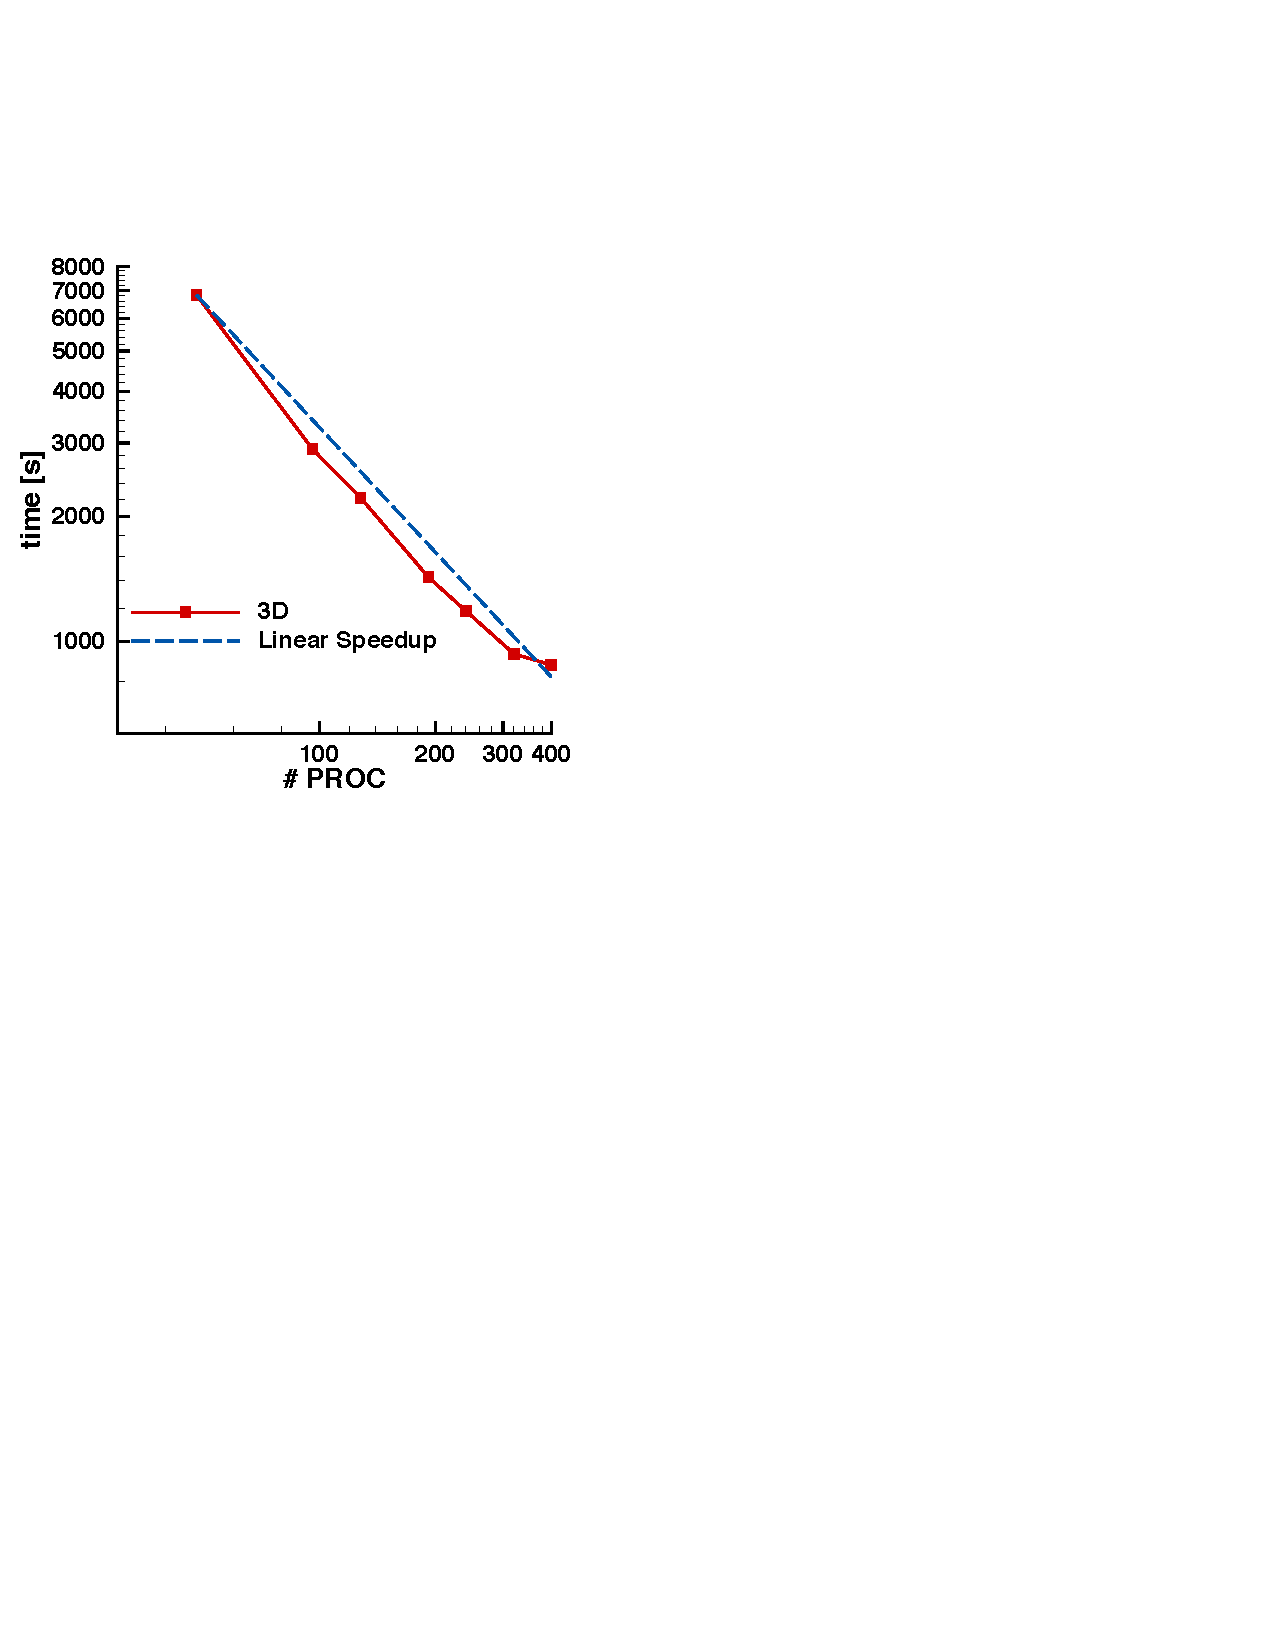
\includegraphics[width=.45\textwidth]{\figpath/Fig_cap_natconv/Scal_ffddm_2level}}
 {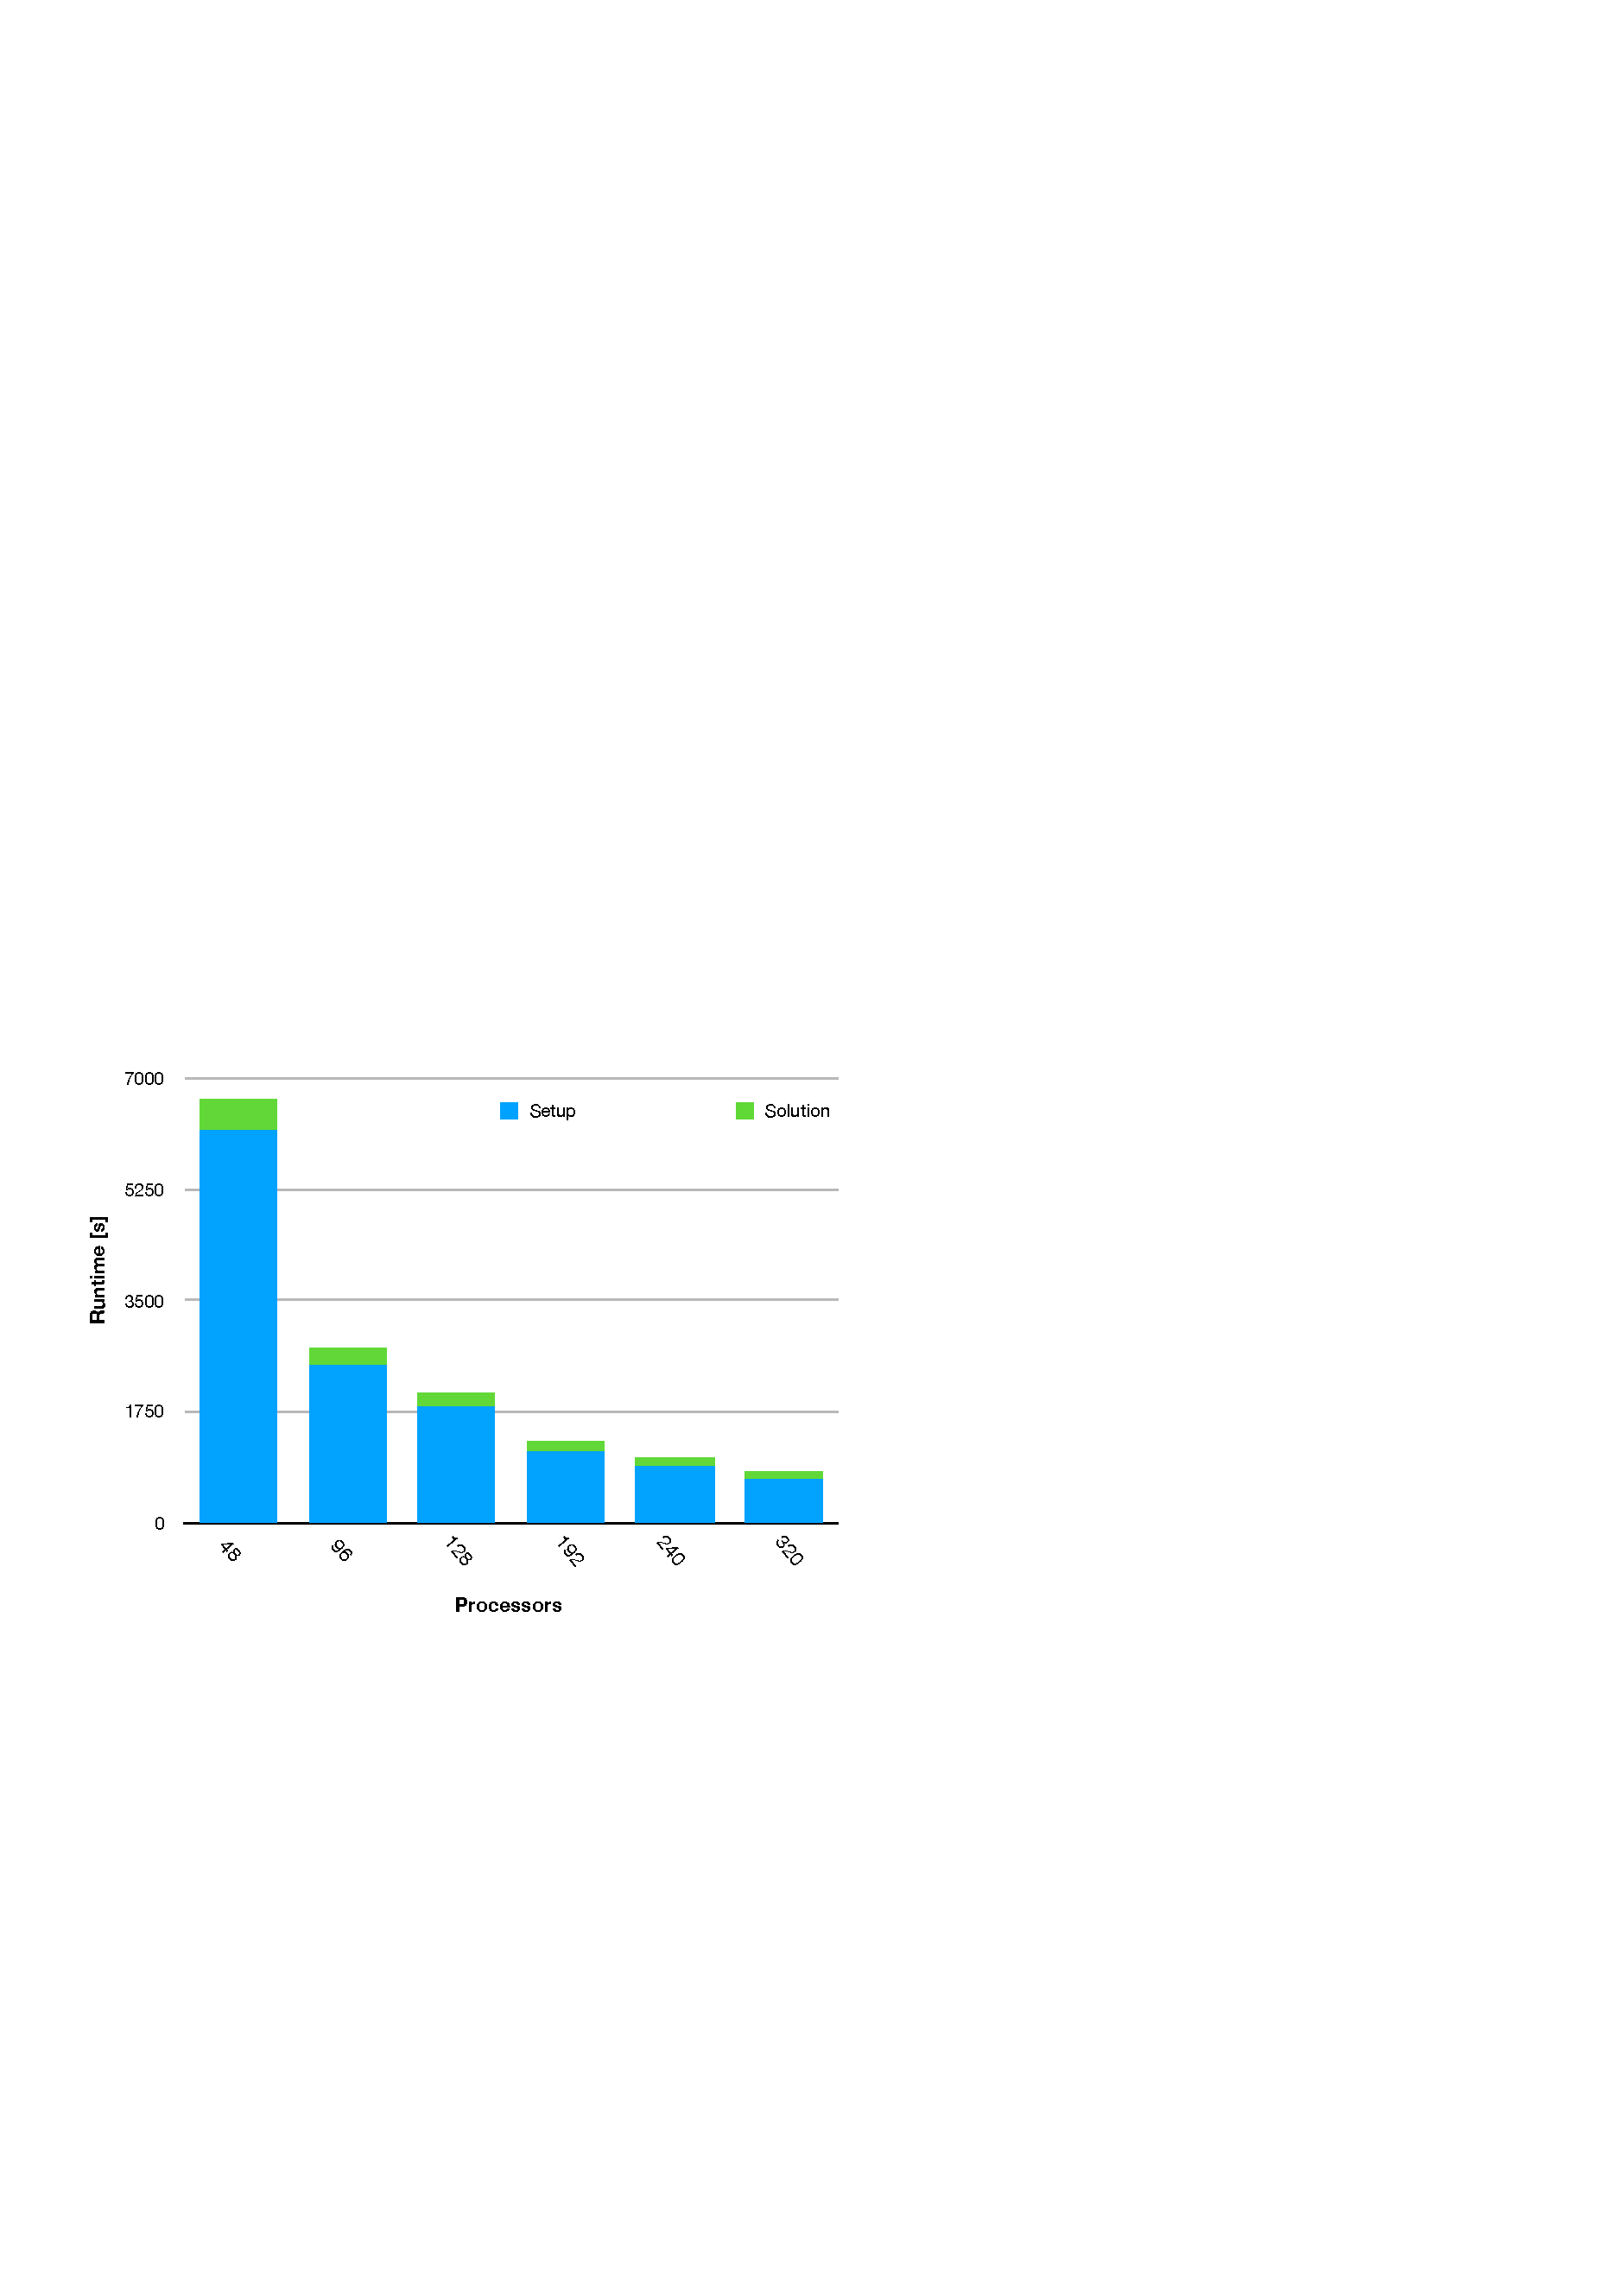
\includegraphics[width=.5\textwidth]{\figpath/Fig_cap_2/scal_ffddm_P2}}
\end{center}
\end{minipage}
\caption{Strong scalability of the ORAS preconditioner: $7.2$ millions of d.o.f and subdomains ranging from $48$ to $400$.}
\label{fig-scalability} 
\end{figure}

\begin{table}[!h]
	\begin{center}
		\begin{tabular}{cccc}
			 $\mathcal{N}$ & Factorization (s)  & GMRES (s)  & Total Step (s) \\ \hline \hline
			 48 & 6186.33  & 473.66  &  6659.99 \\
			 96 & 2468.68  & 283.099 &  2751.779 \\
			 128 & 1814.26 &  237.853 &   2052.113\\
			 192 & 1111.5  &   169.174 &  1280.674 \\
			 240 & 889.422  & 146.539 &  1035.961\\
			 320 & 674.204   &  114.346 & 788.55 \\
			 400 & 614.418  &  107.422 &  721.84\\ \hline
		\end{tabular}
	\end{center}
	\caption {Strong scaling experiment in 3D differentially heated cavity. $7.2$ millions of d.o.f and subdomains ranging from $48$ to $400$. }
	\label{tab-scalability}
\end{table}


